\documentclass[10pt,a4paper]{report}
\usepackage[utf8]{inputenc}
\usepackage[T1]{fontenc}
\usepackage{graphicx}
\usepackage{amsmath}
\usepackage{float}
\usepackage{xfrac}
\usepackage[toc]{glossaries}
\usepackage[font=footnotesize,labelsep=quad]{caption}
\usepackage[toc,page]{appendix}
\PassOptionsToPackage{hyphens}{url}\usepackage[pdfpagelabels]{hyperref}
\setlength{\parskip}{1em}

\newacronym{gui}{GUI}{Graphical User Interface}
\newacronym{flac}{FLAC}{Free Lossless Audio Codec}
\newacronym{png}{PNG}{Portable Network Graphic}
\newacronym{hz}{Hz}{Hertz is the derived unit of frequency in the International System of Units (SI). It is defined as one cycle per second}
\newacronym{khz}{kHz}{Kilohertz, refers to 1000 Hertz}
\newacronym{cdda}{CDDA}{Compact Disc Digital Audio}
\newacronym{mp3}{MP3}{MPEG-2 Audio Layer III, a popular coding format for digital audio}
\newacronym{asic}{ASIC}{Application-specific integrated circuit}
\newacronym{dft}{DFT}{Discrete Fourier Transform}
\newacronym{ntsc}{NTSC}{National Television System Committee, a colour encoding system for analogue television}
\newacronym{pal}{PAL}{Phase Alternating Line, a colour encoding system for analogue television}
\newacronym{db}{dB}{decibel}
\newacronym{dbfs}{dBFS}{decibels relative to full scale}
\newacronym{pcm}{PCM}{Pulse-code modulation, a method used to digitally represent sampled analog signals}
\newacronym{spdif}{S/PDIF}{Sony/Philips Digital Interface}
\newacronym{fpga}{FPGA}{Field-programmable gate array}
\newacronym{wav}{WAV}{Waveform Audio File Format, also referred to as WAVE}
\newacronym{ms}{ms}{Millisecond (\sfrac{1}{1000} of a second)}

%define in parenthesis
\newcommand{\define}[1]{\textit{\acrlong{#1}} (\textit{\acrshort{#1}})}
%define in footnote
%\newcommand{\define}[1]{\textit{\acrshort{#1}\footnote{\textit{\acrlong{#1}}}}}
\newcommand{\defineCite}[2]{\textit{\acrshort{#1}\footnote{\textit{\acrlong{#1}} #2}}}

% shortcuts for the whole document
\newcommand{\ac}[1]{\textit{\acrshort{#1}}}
\newcommand{\hz}[1]{\textit{#1\acrshort{hz}}}
\newcommand{\khz}[1]{\textit{#1\acrshort{khz}}}
\newcommand{\db}[1]{\textit{#1\acrshort{dbfs}}}

\makeglossaries

%opening
\title{MDFourier}
\author{Artemio Urbina}

\begin{document}
	
\pagenumbering{Alph}
\begin{titlepage}
	\maketitle
	\thispagestyle{empty}
\end{titlepage}
\pagenumbering{arabic}

\begin{abstract}
\textit{MDFourier} is an \textit{open source} software solution created to compare \textit{audio signatures} and generate a series of graphs that show how they differ. The software consists of two separate programs, one that produces the signal for recording from the console and the other that analyses and displays the audio comparisons. 

The information gathered from the comparison results can be used in a variety of ways: to identify how \textit{audio signatures} vary between \textit{systems}, to detect if the \textit{audio signals} are modified by \textit{audio equipment}, detect if \textit{modifications} resulted in audible changes, to help tune \textit{emulators}, \ac{fpga} implementations or \textit{mods}, etc.

This document serves as an introduction, a manual and a description of the methods used and how they work. Its intent is to guide new users in making simple comparisons while still providing advanced users with information to perform a more detailed analysis of audio signatures.
\end{abstract}

\tableofcontents

\chapter{Introduction}

\textit{MDFourier} is a free and open source software suite for analyzing and comparing \textit{audio signatures}.

It can be used to identify the differences between two \textit{audio recordings}.  For instance, a \textit{Sega Genesis Model 1 VA3} and a \textit{Sega Genesis Model 2 VA 1.8} can be compared in order to verify how different they are across the human hearing frequency spectrum, using objective and repeatable results.

The process is not limited to one specific system, and the software can be used to compare any other platform by adding new configuration files.\footnote{The term \textit{system} will be used to cover vintage retail hardware, emulators, \ac{fpga} implementations and any other possible variant that executes binaries for the target hardware.} At the moment, profiles for \textit{Mega Drive/Genesis} and \textit{Mega/Sega CD} are functional--with more to follow.

The intention is not to disparage any particular system, but to help understand and improve them whenever possible by identifying their differences.

A secondary but not less important goal is to create a community driven catalog of audio signatures from these systems, in order to help preservation efforts achieve their objectives.

I believe it would be very useful to have configurations tuned to replicate the audio signatures of vintage retail hardware variations in emulators and \define{fpga} implementations. But that doesn't mean there isn't room for improved interpretations; reducing noise while keeping the reference sound signature is one such scenario.

Although powerful industrial solutions for this kind of analysis must exist, they do not seem to have reached the enthusiast community. I'm not aware of any other similar effort to create public software analysis tools that are aimed at vintage console hardware.

It must be noted that there have been detailed comparisons, made in particular for the \textit{MegaDrive/Sega Genesis}.\footnote{See the forum post at \cite{genesisaudio}}. 

\section{Possible applications}

\begin{itemize}
	\item Figure out if \textit{vintage hardware} retail variations really have different audio signatures when compared against each other.
	\item Help emulator and \ac{fpga} implementation authors with tools to tune \textit{filter profiles} that match \textit{vintage retail} hardware audio signatures.
	\item Help the modding community to compare how audio signatures change for each \textit{synthesizer} within the targeted system while developing audio modifications.
	\item Determine if there were changes in the audio \textit{spectrum} after modifications to a console, like \textit{recapping} or changing the audio circuitry.
	\item Evaluate equipment, such as \textit{switchers} and \textit{upscalers} with audio \textit{passthrough}. It can help figure out if they have any effect on the signal, by comparing a recording with and without the device connected in the \textit{Audio/Video} chain.
	\item Help to recreate specific audio signatures.
	\item Help to tune a system to a particular taste.
\end{itemize}


\newpage
\section{Disclaimer}

\textit{MDFourier} and this documentation are a work in progress. Although I tried to adhere to the best practices known to me, my experience in \textit{digital signal processing} was almost non-existent before this project. 

Please contact me if you have corrections, improvements, suggestions or comments. These are encouraged and welcome. Contact information is available in appendix \ref{contact}.

This project was born out of my curiosity to compare the audio signatures of different revisions of the \textit{Mega Drive/Genesis}, and verify them with a tool assisted analysis. Due to my interest in \textit{game preservation} it naturally evolved into its current form, and will hopefully continue to grow.

\chapter{Audio Basics}

This chapter is an introduction to the audio concepts that will be used throughout the document, such as: \textit{frequency}, \textit{amplitude}, \textit{sample rate}, decibel, etc. Hopefully it can provide some insight to those unfamiliar with audio and its \textit{digital representations}.

\section{Sound}

Sound is a series of \textit{vibrations} that travel through a medium. In our case this medium is typically air, but it can be water or even a solid. These vibrations are \textit{waves of pressure} and--as any other \textit{wave}--they have characteristics that we can measure in order to classify and understand them. 

\section{Frequency}

We use the term \textit{frequency} to refer to a repeating event--how \textit{frequent} it is. In this case it means how many times the \textit{wave} we are measuring repeats in a second. We measure this in \textit{cycles per second}, and use a unit named \textit{Hertz} (\ac{hz}). 

As you can imagine these vibrations in the air can have a wide range of \textit{frequencies}, but we can't hear all of them due to biological limitations. The range that humans can typically perceive is called the \textit{human hearing spectrum}. A \textit{spectrum} refers to a continuous range of frequencies, and in this case it is defined to start at \hz{20} and end at \hz{20000}--we commonly use the term \textit{20kiloHertz}, since \ac{khz} refers to multiples of \hz{1000}.\footnote{This is the \textit{decimal-based multiplier} system defined by the \textit{International System of Units} (SI).} These numbers are of course an average, and every one of us has a different \textit{hearing spectrum} that also changes as we age.

In Figure \ref{fig:frequency} we can see a \textit{frequency} of \khz{1} in an audio editor. We can tell it is \textit{1000 cycles per second} since the darker selection spans for \textit{0.01 seconds}, and it has \textit{10} complete \textit{wave cycles} in it.

\begin{figure}[H]
	\centering
	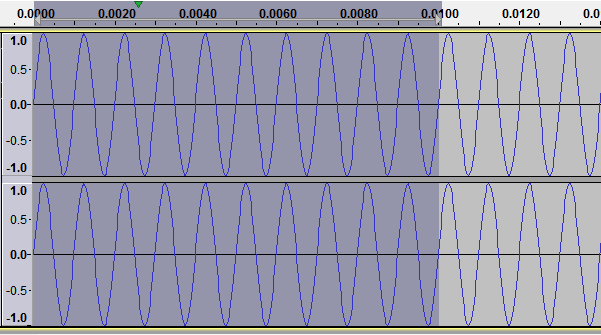
\includegraphics[width=0.8\linewidth]{images/audio/frequency.png}
	\caption[Frequency]{A \khz{1} signal in an audio editor.}
	\label{fig:frequency}
\end{figure}

We perceive \textit{frequency} variations as \textit{pitch differences}: lower \textit{frequencies} are what we call \textit{bass} and higher \textit{frequencies} are \textit{treble}--corresponding to lower and higher \textit{pitched tones}.

\section{Amplitude}

The other \textit{wave} characteristic we use to measure sound is called \textit{amplitude}. This is how \textit{powerful} the \textit{wave} is when compared to the rest of the \textit{signal} that is being analyzed. 

Figure \ref{fig:amplitude} shows a \khz{1} signal that starts at the highest \textit{amplitude} in an audio editor and goes down to zero. This is a typical \textit{fade out}, but done in a very shot period in order to show both \textit{frequency} and \textit{amplitude} in the same image.

\begin{figure}[H]
	\centering
	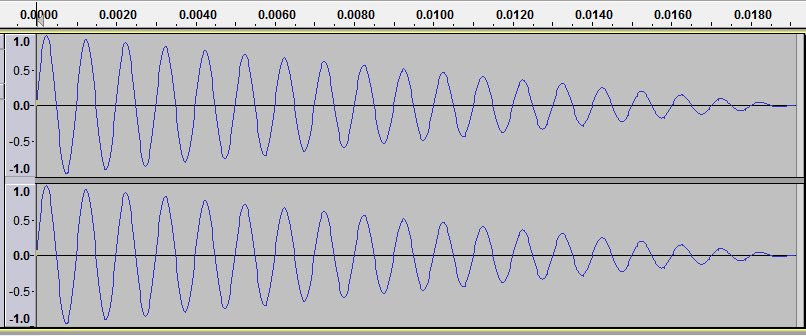
\includegraphics[width=0.8\linewidth]{images/audio/amplitude.png}
	\caption[amplitude]{A \khz{1} signal with gradually lower amplitude.}
	\label{fig:amplitude}
\end{figure}

We perceive this \textit{amplitude} as \textit{volume}, and the terms are directly related. In general, the higher the \textit{amplitude} of a \textit{sound pressure wave}, the higher the \textit{volume} we perceive. But since a sound with the same  \textit{amplitude} but a at another \textit{frequency} can be perceived as a different \textit{volume} by the human ear, the terms don't mean the same thing. Since the software can only use \textit{amplitude} for its calculations, we'll use that term throughout the whole document.

The unit used to measure \textit{amplitude} in \textit{sound pressure waves} is called \define{db}. These use a \textit{logarithmic scale}, which means that in it each subsequent number is a multiple of a base quantity, instead of a sequence of incremental values by a unit as in a \textit{linear scale}. 

We use this scale since it closely models the way we perceive sound, and also because \textit{sound amplitudes} have a very wide range. For instance, the use of a \textit{logarithmic scale} allows us to simultaneously compare the variations of the ambient sound levels from a library against those from a rock concert--even if they are in opposite sides of the \textit{human hearing spectrum}. You might be familiar with this concept from other \textit{logarithmic scales}, like the \textit{Richter scale} used to measure earthquake strength.

Using the scale might be confusing at first, so we'll use an example in order to show how the values behave. Imagine we have two sources that are individually measured as having a \textit{sound pressure level} of \textit{9\acrshort{db}}. If both sources produce sound at the same time, we will measure a combined \textit{sound pressure level} of \textit{12\acrshort{db}} instead of the \textit{18\acrshort{db}} that one might have expected when using a \textit{linear scale}. 

This doesn't mean you'll need to use \textit{logarithm algebra} when dealing with this document--or with sound in general. In practical terms whenever you see a \textit{3\acrshort{db}} difference in sound \textit{amplitude}, it means that you'll perceive \textit{twice} the \textit{volume}.

This scale starts at \textit{0\ac{db}} which is the inferior limit of human hearing, and goes up to \textit{194\ac{db}}; where the sound barrier is broken and it becomes a \textit{shock wave}, at least in the earth's atmosphere. The following table has some common values:\footnote{Table values taken from \cite{noiselevels}--you might notice they are listed as \textit{dBA}, this is tuned to our combined \textit{frequency} and \textit{amplitude} response curve.}

\begin{center}
	\scalebox{0.8}{
		\begin{tabular}{ | r | c | }
			\hline
			\textit{dBA}    & Source\\
			\hline
			0	& healthy hearing threshold\\
			10	& a pin dropping\\
			20	& rustling leaves\\
			30	& whisper\\
			40	& babbling brook\\
			50	& refrigerator\\
			60	& conversational speech\\
			70	& vacuum cleaner at 1 meter\\
			80	& alarm clock\\
			85	& passing diesel truck\\
			90	& squeeze toy\\
			95	& inside subway car\\
			100	& handheld drill\\
			110	& rock band\\
			115	& emergency vehicle siren\\
			120	& thunderclap\\
			125	& balloon popping\\
			130	& peak stadium crowd noise\\
			140	& jet engine at takeoff\\
			145	& firecracker\\
			150	& fighter jet launch\\
			180	& rocket launch\\
			194	& sound waves become shock waves\\
			\hline
		\end{tabular}
	}
\end{center}

\section{Digital representations of sound}

Sound is a continuous signal that varies in time. This means that if you could zoom into it at the smallest fraction of time imaginable, you'd also have a tiny bit of sound happening during that lapse. 

Unfortunately computers don't have the unlimited storage that would be able to replicate a continuous signal--and they also have speed limitations. In order to represent sound in the \textit{digital domain} we use a process called \textit{sampling}. 

\subsection{Sample rate}

\textit{Sampling} involves measuring the \textit{amplitude} of the \textit{sound pressure wave} at \textit{regular cycles}--at a \textit{frequency}--and assigning a value to each one of this measurements. The \textit{frequency} at which we take each of these \textit{samples} from the continuous \textit{audio signal} is called the \textit{sampling rate}. 

The \textit{sample rate} defines the \textit{frequencies} from the signal that we will be able to represent in the digital domain--as the \textit{sampling rate} is increased, so does the \textit{frequency range} that can be portrayed by this digital representation of the signal. 

If we want to represent a certain \textit{frequency range} reliably, we must choose a \textit{sample rate} that is \textit{twice} as big as the highest \textit{frequency} value in the desired \textit{spectrum}.

Since we want to cover the whole \textit{human hearing range}--which goes from \hz{20} to \khz{20}--we must choose a \textit{sample rate} of at least \khz{40}. This is known as the \textit{Nyquist frequency}, and is the reason why some of the most common \textit{sample rates} in digital audio are \khz{44.1} and \khz{48}--which are the ones supported by the \textit{Analysis Software} in \textit{MDFourier}.\footnote{See \cite{MontyMontgomery} for a detailed video demonstration of how \textit{sampling rates} work.}


\subsection{Bit depth}

When we create a \textit{digital representation} of the \textit{amplitude} value for each \textit{sample}, we must define a \textit{bit depth}. This term refers to the amount of \textit{bits}--the minimal piece of data in our current computing systems--that will be used to store each number.

%why 16 and 24 and when they are useful

\subsection{Decibels in the digital domain}

When we were measuring amplitudes before, we used the \ac{db}. In that scenario we were analyzing amplitudes that start at the minimum amplitude our human ears can detect and assigned a value of \textit{0\acrshort{db}} to that level. Values can theoretically go up without limits--aside from that pesky sound barrier we mentioned before when using air as a transmission medium.

However when dealing with digital values that have a defined \textit{bit depth}, our limit is fixed from the other side--the biggest amplitude we can represent with a limited number of \textit{bits}. This number is easily calculated, for \textit{n} bits we get $2^n$ possible values.

Because of this, when using digital files we use a variation of the \textit{decibel} named \define{dbfs}. The highest possible amplitude starts at \db{0} and values go down into negative numbers, until they reach the lowest amplitude that can be represented by the selected \textit{bit depth}. When using a \textit{bit depth} of \textit{16}--as used in \textit{Compact Discs} and by the \textit{Analysis Software} in \textit{MDFourier}--the minimum \textit{amplitude} that can be represented is \db{-96}.

This is commonly referred to as the \textit{dynamic range}, and it tells us now far apart the minimum and maximum \textit{amplitudes} that can be represented in a \textit{audio recording} are. For example, if we have a dynamic range of \textit{96\acrshort{db}}, we can represent the relative amplitudes of \textit{thunderclap} and \textit{rustling leaves} within the same recording; but we could have no lower or higher amplitudes since they'd exceed the range.

%wav
%pcm
%mp3
%flac

\chapter{Working with \textit{MDFourier}}
\label{workflow}

The \textit{software} components that allow \textit{MDFourier} to makes comparisons for a particular platform are:

\begin{itemize}
	\item The \textit{Tone Generator}: It is the piece of \textit{software} that produces the audio signals from the system that is under analysis. 
	\item The \textit{Analysis Software}: This runs on a computer, and creates the graphics that show the results. 
\end{itemize}

The whole process is shown in Figure \ref{fig:mdfourierworkflow}, including the main \textit{hardware} components.

\begin{figure}[H]
	\centering
	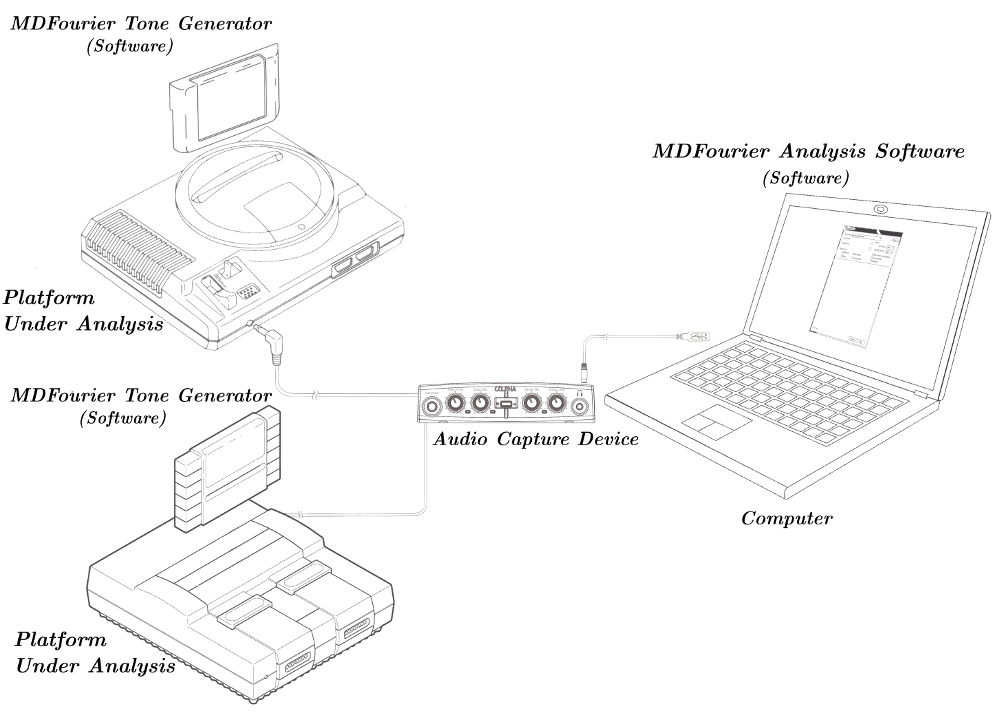
\includegraphics[width=0.8\linewidth]{images/howitworks/MDFourierWorkFlow.png}
	\caption[Workflow]{Relation between the different \textit{hardware} and \textit{software} components of \textit{MDFourier}.}
	\label{fig:mdfourierworkflow}
\end{figure}

\section{Workflow}

The primary thing to keep in mind is what \textit{MDFourier} does. It takes two signals, the first one is designated as the \textit{Reference} file. The second one is the file under scrutiny, and is referred to as \textit{Comparison} file. 

The first step is loading the \textit{Tone Generator} to the desired \textit{system} that will be analyzed. The process for this varies with each platform: from placing the software in a \textit{flash cart}, burning a \textit{CD-ROM} or using a \textit{custom loader}.

The next step is preparing an \textit{audio capture device} and a computer, in order to record an audio file.\footnote{At the moment only 16 bit \ac{wav} and \ac{flac} files with \ac{pcm} encoding and at \khz{44.1 or 48} can be used. \ac{mp3} is not supported, since its compression method alters the results in this type of analysis as shown in section \ref{mp3chap}.} Once the \textit{audio card} is ready, and the cables are hooked up from the \textit{system} to the \textit{audio inputs}, the recording process is started from the \textit{computer} and the \textit{Tone Generator} should be activated from the \textit{system} under analysis.

After a short lapse, usually around one minute, the \textit{Tone Generator} will display a message indicating that the recording process can be stopped. When at least two files are available, one to be used as \textit{reference}--which can be one of the files provided--and one to be used as \textit{comparison} file; a comparison can be made with the \textit{Analysis Software} from the computer.\footnote{All software and some example recordings are available from the web page of the project, see appendix \ref{downloads} for details.}

\section{How \textit{MDFourier} works}

The \textit{Reference} file is used as a control. This means that its characteristics are considered the true values to be expected and against which the \textit{Comparison} file will be evaluated. In consequence, all results are relative between the signals.

Having these files, the software analyzes and compares their audio characteristics and generates graphs that visually show how they differ.

These files are audio recordings from the desired hardware, preferably captured with a \textit{flat frequency} audio \textit{capture card} and produced by a the \textit{Tone Generator} that runs on the target platform.\footnote{Flat frequency response refers to the capability of capturing the whole audible spectrum with little or no variation, regardless of frequency. A non \textit{flat frequency} response card can be used to gather relative information, but the captures won't match the ongoing catalog in order to make further comparisons. See \textit{Audio Cards} in appendix \ref{requirements} for more information.} This \textit{Tone Generator} is specifically crafted for the particular hardware capabilities and frequency range of the target. Whenever possible, the \textit{Tone Generator} will be included in the \textit{240p Test Suite} for the platform to be analyzed.\footnote{A homebrew software suite for video game consoles developed to help in the evaluation of TVs, upscalers, upscan converters, line doublers and video processing in general.\cite{240pSuite}}

Although the \textit{Analysis Software} is \textit{command line} based--in order to be multi-platform and offer the tool on every operating system that has an \textit{ANSI C99 compiler}--a \define{gui} front end for \textit{Microsoft Windows} is provided for simplicity and accessibility.\footnote{See appendix \ref{usinggui} for a guide on how to use the software.} Full Source code can be downloaded from \textit{github}.\footnote{See download link \cite{sourcecode}.}

\section{File alignment}

\textit{MDFourier} takes both files and auto detects the starting and ending points of the recording. These are identified by a series of \hz{8820} pulses in the current \textit{Mega Drive/Genesis} implementation. From these, a \textit{frame rate}\footnote{The \textit{frame rate} is the ratio at which the console sends video frames to a display. For more details see appendix \ref{framerate}} is calculated in order to trim each file into the segments that are defined in the \textit{configuration file}\footnote{This file specifies the operating parameters for each hardware configuration. It is described in appendix \ref{mfnconfig}} for further comparison.

Most importantly, it guarantees that the \textit{Reference} and \textit{Comparison} files are logically aligned, and that each note--or segment--is compared to its corresponding one, with no overlap and without any audio editing or trimming skills required from the user. Current pulse detection accuracy is around $\sfrac{1}{4}$ of a millisecond.

After alignment is accomplished, the software reports the starting and end points of both signals, in seconds and bytes.

\section{The heart of the process}

A process called \textit{Discrete Fourier Transform}\footnote{\gls{dft} is the variant of \textit{Fourier Transform} applied to discrete values, such as the ones we have in the audio file. See \cite{FourierTransformApps}.} is used in order to analyze and compare the \textit{amplitudes} from each of the \textit{frequencies} and \textit{harmonics}--the \textit{spectrum}--that compose the audio signal. The software uses the \textit{FFTW}\footnote{\textit{The Fastest Fourier Transform in the West.} \cite{fftw}} library in order to accomplish this.

In order to compare the frequencies and amplitudes of each file against each other, a reference point must be set. This is achieved via a relative \textit{normalization}\footnote{This process is detailed in appendix \ref{normalization}.} based on the \textit{maximum amplitude} of the \textit{Reference} file. A \textit{local} maximum search is done at the same frame in the \textit{Comparison} signal, and that amplitude is then used to normalize both files. 

This is done in the \textit{frequency domain}\footnote{Basically all analysis from this point and forward takes place after the signal has been decomposed into its fundamental and harmonic sine waves by the Fourier Transform.}, in order to reduce amplitude imprecision when comparing recordings with different \textit{frame rates}\footnote{For more details see appendix \ref{framerate}.}. The software does have the option to do this in the \textit{time domain}\footnote{In other words, normalize based on the samples and their values. This is detailed in appendix \ref{normalization}.}, but quantization and amplitude imprecision is to be expected if used.

After normalization is finished, the frequencies of each \textit{block}\footnote{A \textit{block} is the basic segment of audio to be compared, such a specific note by a synthesizer as generated by the \textit{Tone Generator}.} are sorted out by amplitude, from highest to lowest. \textit{MDFourier} can be configured to compare a range of these frequencies--by default \textit{2000} of them are compared for each \textit{block} defined in the \textit{mfn} configuration file\footnote{Described in appendix \ref{mfnconfig}.}. I've found such number to be more than enough, and usually the \textit{minimum significant amplitude}\footnote{See section \ref{MinSigAmplitude}.} limits this parameter to an even lower number. In case a a different comparison of frequencies is needed, the amount can be increased or decreased via the command line\footnote{See appendix \ref{extracommand}.}.

Sometimes it is helpful to listen to the results of these limiting filters, in order to evaluate if --for instance--\textit{2000} frequencies are either enough or too little for the current application. For this and other purposes I made an extra tool named \textit{MDWave}\footnote{Described in appendix \ref{mdwave}.}, which creates segmented audio files as internally processed by \textit{MDFourier}, even including the effects of \textit{window}\footnote{Window functions are described in section \ref{windows}.} filters and amplitude limits.

After comparing these frequencies between both files, matches are made and the differences in amplitude are plotted to a graph. Please read chapter \ref{howtographs} for a detailed description of what the various graphs created by the program represent.

If you are interested in learning what the \textit{Fourier Transform} does and how its \textit{"magic"} works, there are several resources online. Here are a few of them:

\begin{itemize}
	\item But what is the Fourier Transform? A visual introduction.\\ \url{https://www.youtube.com/watch?v=spUNpyF58BY}
	\item An Interactive Introduction to Fourier Transforms.\\ \url{http://www.jezzamon.com/fourier/}
	\item The Uncertainty Principle and Waves.\\ \url{https://www.youtube.com/watch?v=VwGyqJMPmvE}
\end{itemize}

\section{Minimal significant amplitude}
\label{MinSigAmplitude}

Although the whole frequency spectrum can be compared, there is little practical use in doing so--due to execution time and extra noise from low amplitude harmonics. As a result, rule of thumb defaults are set in order to minimize these issues.

One of these values is a \textit{minimum amplitude} at which to stop comparing the fundamental frequencies that are found after decomposing the signal with the \textit{Fourier Transform}. This is the \textit{minimal significant amplitude} and it is the cutoff at which comparisons made by the software are stopped.

Currently \textit{MDFourier} can recognize three scenarios to define the \textit{minimal significant amplitude} to compare the signals, and the three are derived from the first \textit{silence block} in the file.

The first scenario is the \textit{electrical grid} frequency noise, which is searched for at either \hz{60} for \ac{ntsc} or \hz{50} for \ac{pal}.\footnote{\ac{pal} needs to be tested yet, since I don't have console for that video system.} This is automatically selected from the previously calculated \textit{frame rate}, if available.

The second one is \textit{refresh rate noise}, again derived from the frame rate, in \ac{ntsc} it is between \hz{15697-15698}. 

If neither is found, which would be surprising for a file generated by recording from a vintage console via analogue means, the frequency with the highest amplitude within the \textit{silence block} is used. 

Finally, in case none of the previous scenarios is met--or if those values are lower than \db{-60}--a default level of \db{-60}\footnote{This can be changed via \textit{command line} options if needed. See appendix \ref{extracommand}.} is used. 

\chapter{How to interpret the graphs}
\label{howtographs}

The main output of the program is a set of different graphs that vary in quantity based on the definitions made in the \textit{mfn} file\footnote{Detailed in appendix \ref{mfnconfig}.}, and the selected options\footnote{See appendix \ref{usinggui}.}.

The graph files are saved under the folder \textit{MDFourier} and a sub-folder named after the input \ac{wav} file names. They are stored in \define{png} format. Currently \textit{1600x800} graphs are used, although this can be changed via options. 

For the current document \textit{800x400} graphs were used in order to fit within a \textit{PDF} or \textit{HTML} presentation. The output graphs that are created by the software are listed and described in appendix \ref{outputfiles}.

In our examples for the \textit{Mega Drive/Genesis}, there are three \textit{active blocks}\footnote{\textit{The Mega Drive/Sega Genesis} has two audio synthesizers: a \textit{Yamaha 2612} (YM2612) for \textit{Frequency Modulated} (FM) audio, and a \textit{Texas Instruments SN76489 Programmable Sound Generator} (PSG)--or equivalent in an \ac{asic}--for \textit{Sega Master System} compatibility and extra audio channels.}: \textit{FM}, \textit{PSG} and \textit{Noise}. These will result in a graph of each type, plus a general one named \textit{ALL}.

We'll follow a series of results from different input files to \textit{MDFourier}, starting with cases that have either none or a few differences and build on top of each one, so you can familiarize with what to expect as output.

\section{Scenario 1: Comparing the same file against itself}
\label{scenario1}

The first scenario we'll cover is the basic one, the same file against itself. Let's keep in mind that \textit{MDFourier} is designed to show the relative differences between two audio files.

So, what is the expected result of comparing a file to itself? No differences at all. An empty graph file as shown in figure \ref{fig:plot1-samefile}.

\begin{figure}[H]
	\centering
	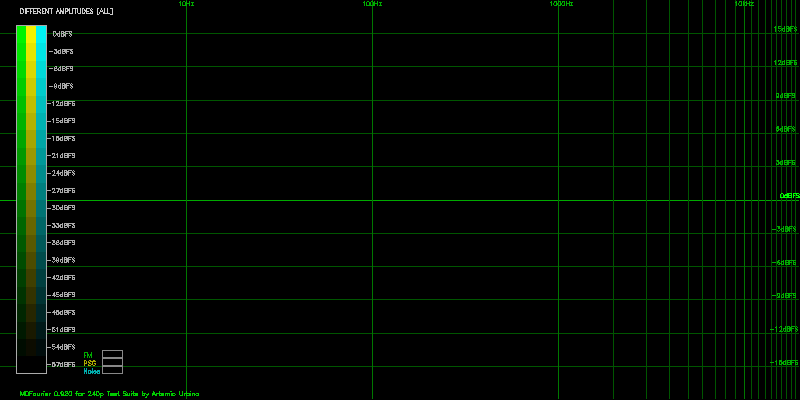
\includegraphics[width=1.0\linewidth]{images/interpretation/Plot1-SameFile.png}
	\caption[Same file compared]{Different Amplitudes result file when comparing the same file against itself.}
	\label{fig:plot1-samefile}
\end{figure}

Of course all of the \textit{Differences} and \textit{Missing} graphs will only have the grid and reference bars, with no plotted information since both input files are identical.

All graphs use the horizontal axis for frequency. Values start from \hz{1} on the left and end at  \khz{20} on the right, which covers the human hearing spectrum\footnote{Although the plotted range can be altered to cover only a fraction of the spectrum, the resulting graph will hold the same scale.}.

For \textit{Difference} graphs the vertical axis is the amplitude in \ac{dbfs}, and a central axis for \db{0}. Values rise to \db{18} towards the top and fall to \db{-18} on the lower part of the graph.

There will be two sets of \textit{Spectrograms}, one for the \textit{Reference} file and one for the \textit{Comparison} file, with one graph for each defined \textit{type} plus the general one.

\begin{figure}[H]
	\centering
	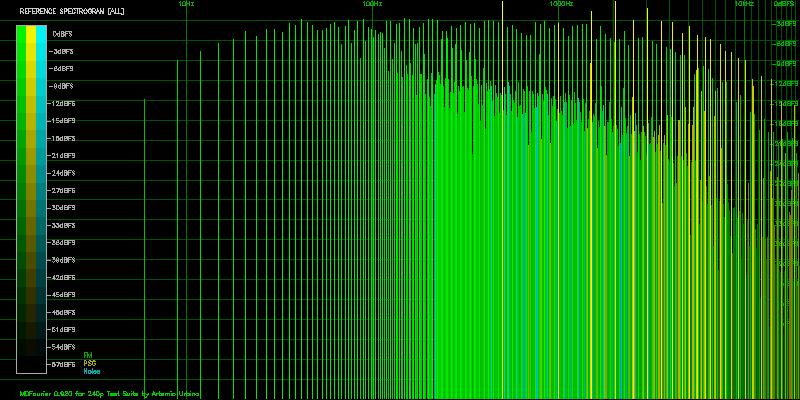
\includegraphics[width=1.0\linewidth]{images/interpretation/Plot1-SameFile-Spectrogram.png}
	\caption[Spectrogram]{The Spectrogram for a Genesis 1 VA3 via headphone out.}
	\label{fig:plot2-samefile-fm-spectrogram}
\end{figure}

The Amplitude of each of the fundamental \textit{sine waves} that compose the original signal is represented by vertical lines that reach from the bottom to the point that corresponds to the amplitude in \ac{dbfs}. The line is also colored to represent that amplitude with the scale on the left showing the equivalence.

Three colors--as defined from the \textit{mfn file}\footnote{The configuration file is described in appendix \ref{mfnconfig}.}--are used to plot the graph, with each one of them plotting the frequencies from each corresponding \textit{type} from the \ac{wav} file.

The top of the graph corresponds to the maximum possible amplitude, which is \db{0}. The bottom of the graph corresponds to the \textit{minimum significant amplitude}, as described in section \ref{MinSigAmplitude}.

As expected, both sets of \textit{spectrograms} are identical in this case, since we used the same file compared against itself.

\section{Scenario 2: Comparing two different recordings from the same console}
\label{scenario2}
This is another control case. What should we expect to see if we record two consecutive audio files from the same console using the same sound card?

\begin{figure}[H]
	\centering
	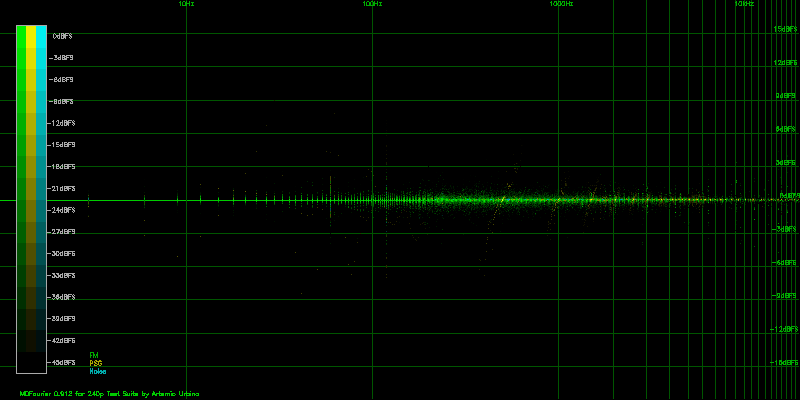
\includegraphics[width=1\linewidth]{images/interpretation/Plot2-Sameconsole.png}
	\caption[Same console compared]{The same console, two different recordings.}
	\label{fig:plot2-sameconsole}
\end{figure}

As you can see, we have basically a flat line around zero. This means that there were no meaningful differences found. 

But wait, there \textit{are} differences. Why is that? Due to many reasons: analogue recordings are not always identical. There are also variations from the analogue part of console itself, and probably from the internal states and clocks from the digital side of the process. It can also be noise generated by differences in frequency bins when performing the \define{dft} after calculating the frame rates--we have that $\sfrac{1}{4}$ alignment error after all.

We now know that there will be certain \textit{fuzziness}, or variation, around each graph due to this subtle recording and performance nuances. It is a normal situation that is to be expected, and a baseline for further results.

\begin{figure}[H]
	\centering
	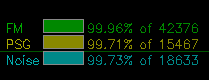
\includegraphics[width=0.4\linewidth]{images/interpretation/Plot2-Sameconsole-bars.png}
	\caption[Bars]{Bars for percentage matched.}
	\label{fig:plot2-sameconsole-bars}
\end{figure}

Until now we haven't discussed the small bars at the lower left quadrant of the graphs. These represent the percentage of matches that were made. In this case we get all above 99.8\% as shown in figure \ref{fig:plot2-sameconsole-bars}. This serves as a quick guide on how relevant the plotted differences are when comparing both signals. The numbers to the right\footnote{Only drawn at higher resolutions, since they aren't readable in 600x400 mode.} is the amount of values that were compared.

\section{Scenario 3: Comparing against a modified file}
\label{scenario3}

For demonstration purposes, the same \textit{Reference} file was modified to add a \hz{500} \db{6} parametric equalization across all the signal. This is an artificially modified and controlled scenario in order to demonstrate what the graphs mean.

\begin{figure}[H]
	\centering
	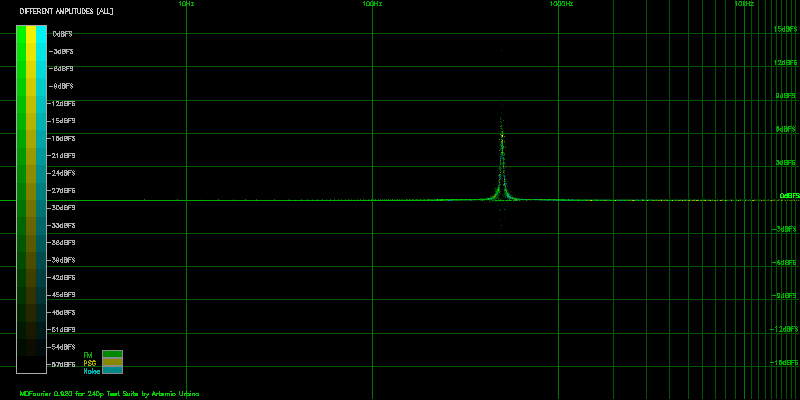
\includegraphics[width=1.0\linewidth]{images/interpretation/Plot3-Modified.png}
	\caption[1kHz modified]{Compared against itself modified with a \hz{500} \db{6} equalization.}
	\label{fig:plot3-modified}
\end{figure}

As expected all three \textit{types} (\textit{FM}, \textit{PSG} and \textit{Noise}) were affected and show a spike, exactly \db{6} tall and centered around \hz{500}.

It is interesting to contrast both spectrograms (figures \ref{fig:plot3-spectrogram} and \ref{fig:plot3-spectrogram-500Hz}), since the \hz{500} spike is also shown there.

\begin{figure}[H]
	\centering
	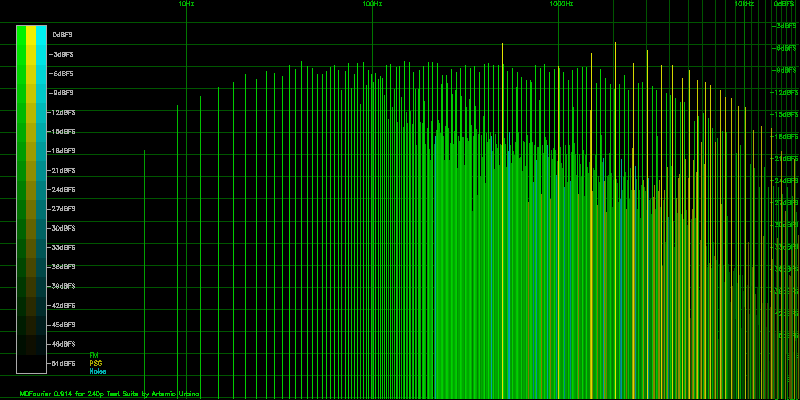
\includegraphics[width=1.0\linewidth]{images/interpretation/Plot3-Spectrogram.png}
	\caption[Reference File]{Spectrogram for the \textit{Reference} File.}
	\label{fig:plot3-spectrogram}
\end{figure}

\begin{figure}[H]
	\centering
	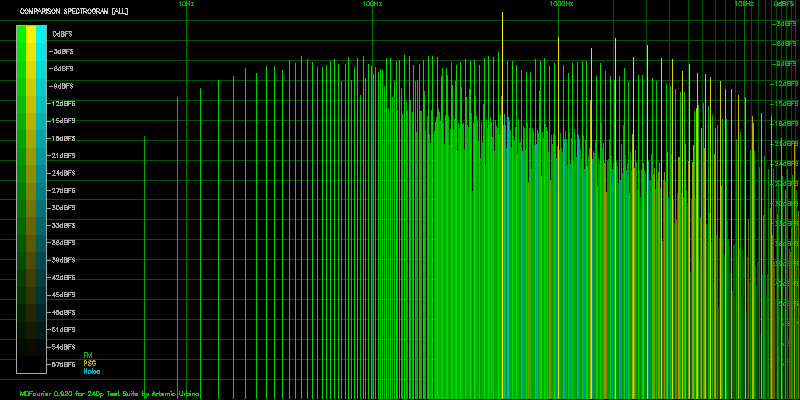
\includegraphics[width=1.0\linewidth]{images/interpretation/Plot3-Spectrogram-500hz.png}
	\caption[Reference File]{\textit{Comparison} file modified with \hz{500} peak.}
	\label{fig:plot3-spectrogram-500Hz}
\end{figure}


And the \textit{Missing Frequencies} graphs are basically empty, since no relevant frequencies are missing from the \textit{Comparison} file.

\section{Scenario 4: Comparing against digital low pass and high pass filters}

We will use the same \textit{Reference} file, and compare it to a file modified by several digital filters that were inserted via an audio editor:

\begin{itemize}
	\item A \textit{low pass filter}\footnote{A \textit{low pass filter} allows only frequencies. lower than a specified value pass through.} to the \textit{FM} section of the file.
	\item A steeper \textit{low pass filter} at a different cutoff frequency to the \textit{PSG} section.
	\item A \textit{high pass filter}\footnote{A \textit{high pass filter} allows only frequencies. higher than a specified value pass through.} to the \textit{Noise} section at a different frequency.
\end{itemize}

Figure \ref{fig:plot4-1-all} shows the general graph for the three types:

\begin{figure}[H]
	\centering
	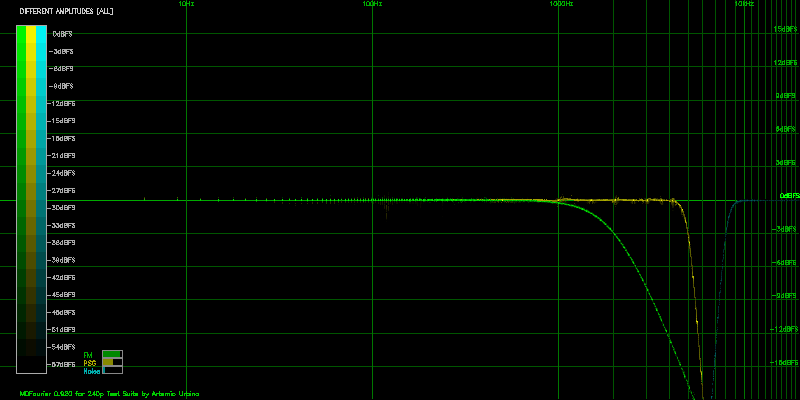
\includegraphics[width=1.0\linewidth]{images/interpretation/Plot4-1-All.png}
	\caption[All Plotted]{\textit{FM} with a low pass filter (in green), \textit{PSG} with a low pass filter (in yellow) and \textit{Noise} with a high pass filter (in aqua).}
	\label{fig:plot4-1-all}
\end{figure}

We can now see that the higher frequencies above \khz{1} in the \textit{FM} graph quickly fall down towards \db{$-\infty$}, so the first low pass filter is there.

The second low pass filter for \textit{PSG} is at \khz{3}, and it is steeper.

But we can barely see what is going on with the \textit{Noise} part of the graph. We can see that there is some black dots on top of the \db{0} line.

In order to better see what is going on, we'll change the \textit{color filter function} to $\sqrt{\ac{dbfs}}$ so we can have higher contrast against the background.\footnote{Described in appendix \ref{colorfilter}.}

\begin{figure}[H]
	\centering
	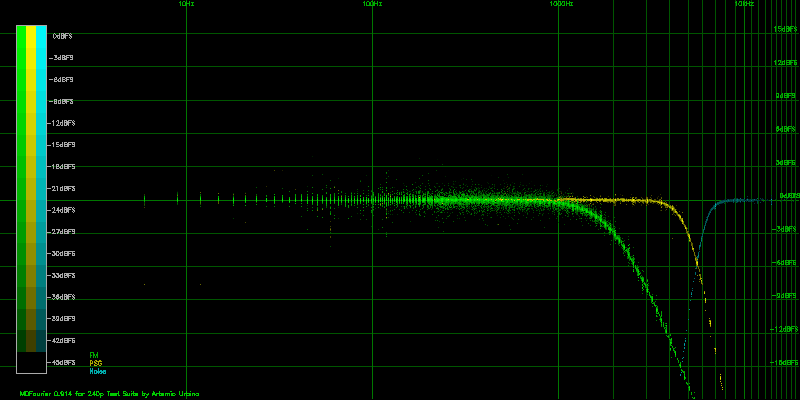
\includegraphics[width=1.0\linewidth]{images/interpretation/Plot4-2-All-sqrt.png}
	\caption[Using SQRT]{Using the $\sqrt{\ac{dbfs}}$ color filter function.}
	\label{fig:plot4-2-all-sqrt}
\end{figure}

With the new emphasis, we can now make out the curve that raises from \db{$-\infty$} to \db{0}, and it aligns with \khz{8}.

We can still do better than that, by using the \textit{Average Graphs} option.\footnote{See section \ref{usinggui} for details.}

Here is the resulting graph for only the \textit{Noise} section of the signal, with average enabled:

\begin{figure}[H]
	\centering
	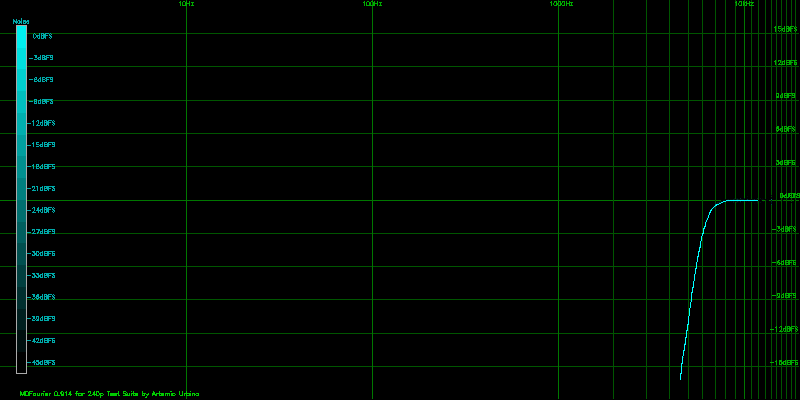
\includegraphics[width=1.0\linewidth]{images/interpretation/Plot4-3-AVG-Noise.png}
	\caption[Noise Average]{\textit{Noise} plot with the \textit{Average Graphs} option enabled.}
	\label{fig:plot4-3-avg-noise}
\end{figure}

There are some other interesting graphs that result from this experiment. For example, the \textit{Missing} graphs now show all the frequencies the \textit{low/high pass} filters cutoff.

\begin{figure}[H]
	\centering
	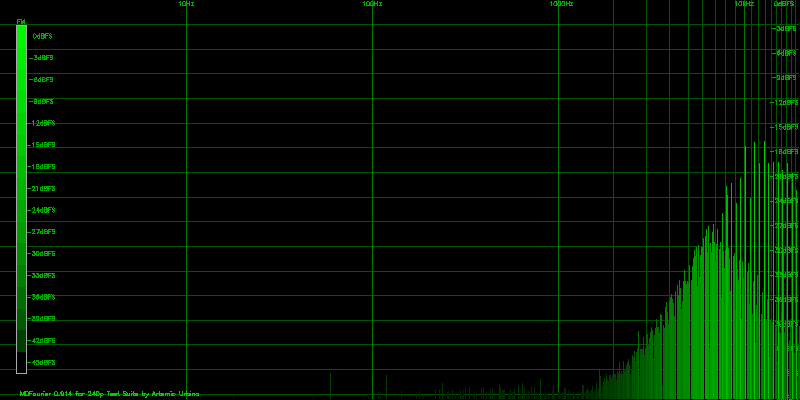
\includegraphics[width=1.0\linewidth]{images/interpretation/Plot4-4-Missing-FM.png}
	\caption[Missing FM]{Missing frequencies in \textit{FM} cutoff by low pass filter.}
	\label{fig:plot4-4-missing-fm}
\end{figure}

As show in Figure \ref{fig:plot4-4-missing-fm}, there is a curve in the \textit{spectrogram} and only frequencies above \khz{1} show up, slowly rising in amplitude. Many of these are not shown since they are below our defined \textit{minimum significant amplitude}.

\begin{figure}[H]
	\centering
	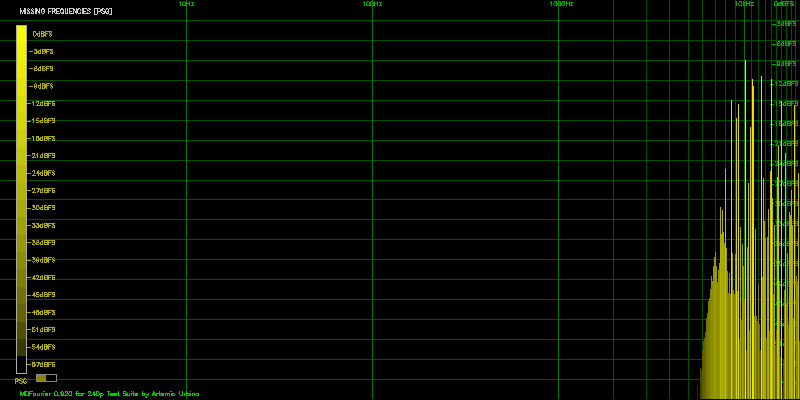
\includegraphics[width=1.0\linewidth]{images/interpretation/Plot4-5-Missing-PSG.png}
	\caption[Missing PSG]{Missing frequencies in \textit{PSG} cutoff by low pass filter.}
	\label{fig:plot4-5-missing-psg}
\end{figure}

The same behavior can be observed in in Figure \ref{fig:plot4-5-missing-psg}. This is the \textit{PSG spectrogram}, and it shows a different curve that starts at \khz{4}. 

As you might have noticed, a bar is also present in the \textit{Missing graph}. But in this case it represents the percentage of unmatched frequencies, as shown in Figure \ref{fig:plot4-5-missing-psg-bars}.

\begin{figure}[H]
	\centering
	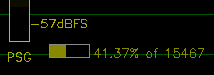
\includegraphics[width=0.4\linewidth]{images/interpretation/Plot4-5-Missing-PSG-bar.png}
	\caption[Missing PSG Bar]{Bar for missing frequencies in \textit{PSG} cutoff by low pass filter.}
	\label{fig:plot4-5-missing-psg-bars}
\end{figure}

And finally, figure \ref{fig:plot4-6-missing-noise} shows the opposite kind of curve, the \textit{high pass filter} that cuts off everything higher than \khz{8} in the \textit{Noise} section.

\begin{figure}[H]
	\centering
	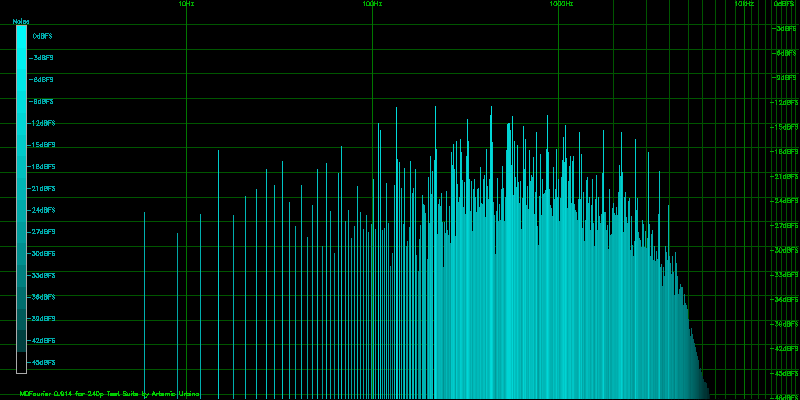
\includegraphics[width=1.0\linewidth]{images/interpretation/Plot4-6-Missing-Noise.png}
	\caption[Missing Noise]{Missing frequencies in \textit{Noise} cutoff by high pass filter.}
	\label{fig:plot4-6-missing-noise}
\end{figure}

It is a good moment to emphasize that these are relative graphs. They show how different the \textit{Comparison} signal is to the \textit{Reference} signal. And so far we've compared the same signal to itself, although modified though very precise digital manipulations. An analog filter would look the same, but a bit fuzzier. 

However, some interesting ideas arise. What would happen if we take this \textit{low/high pass filter} signal and use it as \textit{Reference} and the original one as \textit{Comparison}?

\begin{figure}[H]
	\centering
	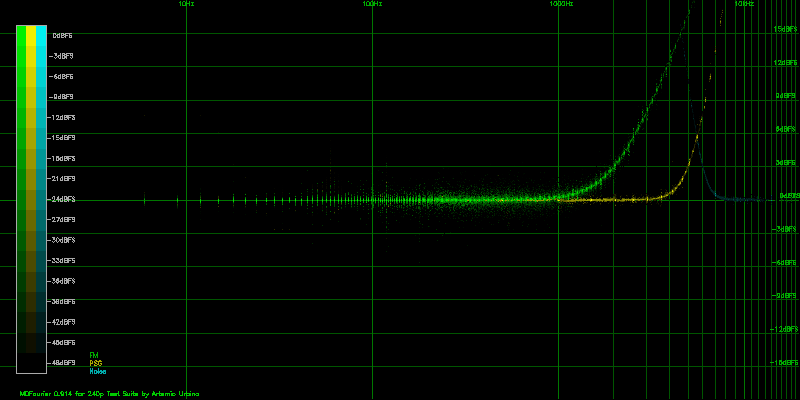
\includegraphics[width=1.0\linewidth]{images/interpretation/Plot4-7-Reversed.png}
	\caption[Reversed]{Results when using modified signal as \textit{Reference}.}
	\label{fig:plot4-7-reversed}
\end{figure}

Based on this, one could jump to the conclusion that everything will simply be inverted. After all, the original signal now rises to \db{$+\infty$} at the same spots--and that makes complete sense--since those frequencies now have a higher amplitude. 

Although the \textit{Differences} graphs will indeed be inverted under these controlled conditions, the \textit{Missing} graphs are different. Most of them are now empty:

\begin{figure}[H]
	\centering
	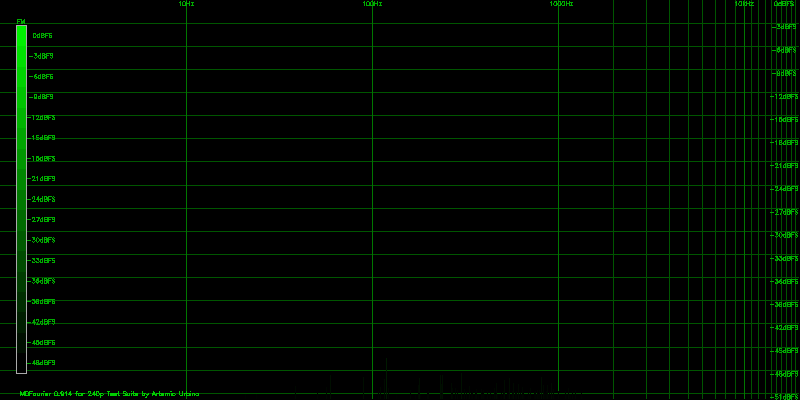
\includegraphics[width=1.0\linewidth]{images/interpretation/Plot4-8-Missing-FM-Inverted.png}
	\caption[Reversed FM Missing]{\textit{Missing Frequencies} graph for \textit{FM} is empty.}
	\label{fig:plot4-8-missing-fm-inverted}
\end{figure}

This happens because although we cut a lot of frequencies with such steep \textit{low} and \textit{high pass filters}, all the frequency content from this modified signal is present in the original, but not the other way around as shown above.

\section{Scenario 5: Comparing two recordings from the same console made with different Audio Cards}

We'll now compare the same console using two different recordings, one made with the \textit{USB Lexicon Alpha} and the other with a \textit{USB M-Track}\footnote{See appendix \ref{audiocards} for details on the sound cards used.}. Figure \ref{fig:plot5-1-all} shows the results:

\begin{figure}[H]
	\centering
	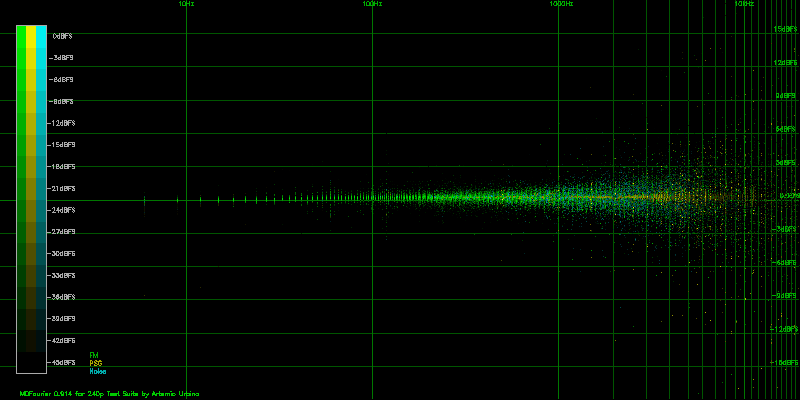
\includegraphics[width=1.0\linewidth]{images/interpretation/Plot5-1-All.png}
	\caption[Different sound cards]{Differences using same system and cables, but different audio capture cards.}
	\label{fig:plot5-1-all}
\end{figure}

There is some scatter, as it was to be expected from the results of \textit{Scenario 2}\footnote{See section \ref{scenario2}.}. We can tell that the scatter is centered around the \db{0} line, which means that even using different sound cards we discern differences between systems\footnote{Under the assumption both cards have a relatively flat frequency response, like the ones used here. For specifications see the \textit{Audio Cards} appendix \ref{audiocards}.}. 

Also, there was a slight difference in the detected frame rates. This happens since the sampling clock is not exactly the same in both audio cards\footnote{More information in appendix \ref{samplingclocks}.}. Here is the output text from the analysis that shows the detected frame rates:

\begin{verbatim}
* Loading 'Reference' audio file A-MD1UTVA3-LA.wav
- WAV file is PCM 48000Hz 16bits and 63.76 seconds long
- Starting sync pulse train:  1.88142s [361232 bytes]
- Trailing sync pulse train:  60.2921s [11576080 bytes]
- Detected 59.9204 Hz video signal (16.6888ms per frame) from WAV file

* Loading 'Comparison' audio file A-MD1UTVA3-MT.wav
- WAV file is PCM 48000Hz 16bits and 62.5774 seconds long
- Starting sync pulse train:  1.44967s [278336 bytes]
- Trailing sync pulse train:  59.8602s [11493160 bytes]
- Detected 59.9208 Hz video signal (16.6887ms per frame) from WAV file

- Reference signal stereo imbalance: left channel is higher by 0.570059%
- Comparison signal stereo imbalance: right channel is higher by 0.487369%
\end{verbatim}

At \khz{48} both cards have very accurate sampling clocks with a minimal difference\footnote{We are talking \textit{0.0001}\ac{ms}. In this case, that is \textit{0.0000001 seconds}!} and \textit{MDFourier} compensates for such issues.\footnote{The expected frame rate from the vintage console analyzed here is \textit{16.688}\ac{ms} per frame, or \hz{59.92} as measured with a scope. See appendix \ref{framerate}} Differences can be more prominent when using \khz{44.1}, but the software can still compensate for them without issues.

Here is the graph with the \textit{Average Graphs} option turned on:

\begin{figure}[H]
	\centering
	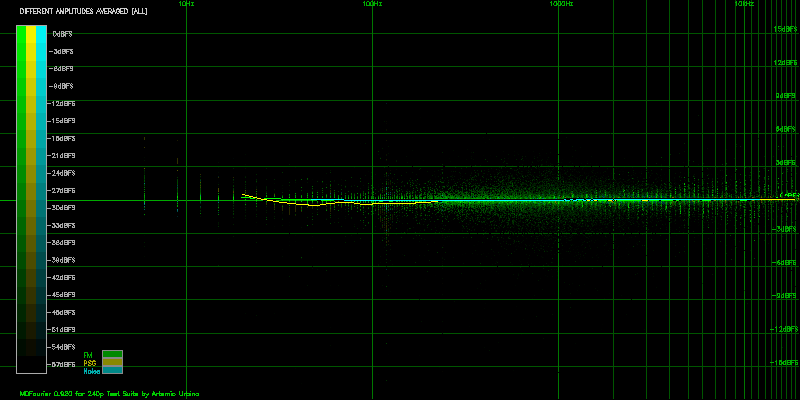
\includegraphics[width=1.0\linewidth]{images/interpretation/Plot5-2-avg.png}
	\caption[Different sound cards AVG]{Differences using same hardware and cables, different capture cards with average enabled.}
	\label{fig:plot5-2-avg}
\end{figure}

The results obtained are quite similar to the ones from \textit{scenario 2}, even to the point of getting almost the same percentages as shown in Figure \ref{fig:plot5-3-bars}. So as long as we are using a relatively flat frequency response audio card, we'll be able to compare results from different systems even when using a variety of audio cards.

\begin{figure}[H]
	\centering
	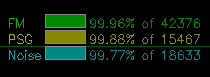
\includegraphics[width=0.4\linewidth]{images/interpretation/Plot5-3-bars.png}
	\caption[Different sound cards Bars]{Percentage match Bars using same hardware and cables, different capture cards.}
	\label{fig:plot5-3-bars}
\end{figure}

\section{Scenario 6: Comparing \textit{WAV} vs \textit{MP3}}
\label{mp3chap}

The audio file from \textit{Scenario 1} will be used as \textit{Reference} and \textit{Comparison} file, but this time encoded as \ac{mp3}\footnote{The file was created with the \textit{MP3 LAME} encoder using \textit{variable bit rate} in high quality mode, with slow encoding enabled and using real stereo.} and decompressed to \ac{wav} in order to use it with the software.

If the files were identical, an empty graph would result as shown in Figure \ref{fig:plot1-samefile} from \textit{Scenario 1}. However we get something slightly different:

\begin{figure}[H]
	\centering
	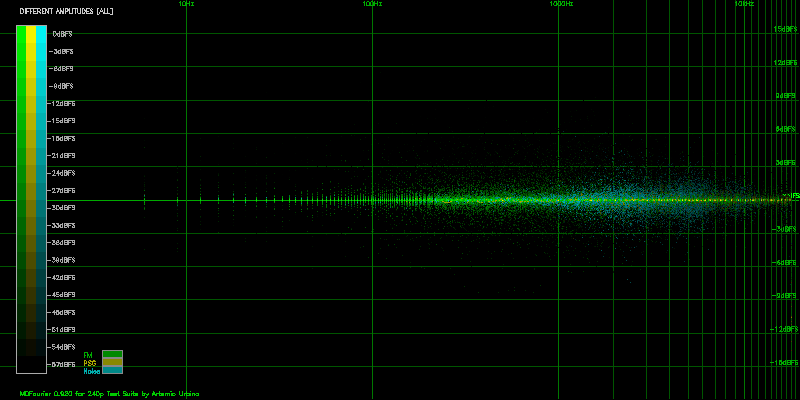
\includegraphics[width=1.0\linewidth]{images/interpretation/Plot6-mp3-1.png}
	\caption[WAV vs MP3]{Differences between \ac{wav} as \textit{reference} and \ac{mp3} as \textit{Comparison}.}
	\label{fig:plot6-mp3-1}
\end{figure}

We get everything centered around the \db{0}--as it should be--which indicates the \textit{audio signatures} are very similar. Variations are correspondent to what we found in \textit{Scenario 5} while we were comparing the same console with different audio cards. It must be noted that we used high quality compression for the test, and lower settings will provide different results. The reader is invited to experiment with the tools.

However in this case some more differences show up if we enable the \textit{Average Graphs} option:

\begin{figure}[H]
	\centering
	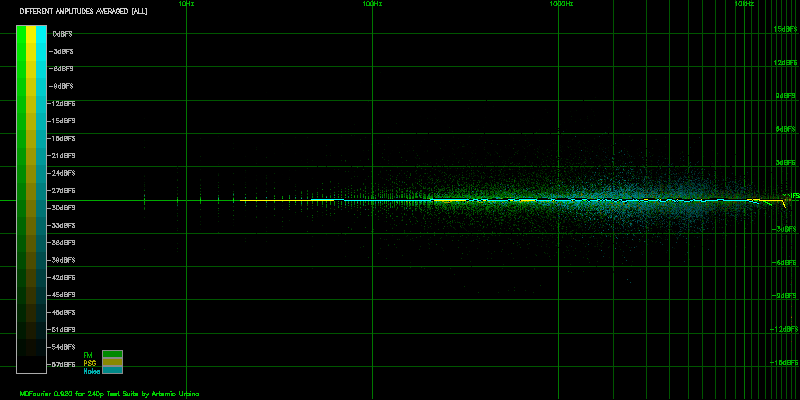
\includegraphics[width=1.0\linewidth]{images/interpretation/Plot6-mp3-2.png}
	\caption[WAV vs MP3 Averaged]{Differences between \ac{wav} as \textit{reference} and \ac{mp3} as \textit{Comparison}, averaged.}
	\label{fig:plot6-mp3-2}
\end{figure}

As it can be appreciated in the rightmost part of the graph, there is a low pass filter around \khz{18}. These frequencies are at the border of acoustic human limits, and most adults won't even be able to hear them. In part this is what \ac{mp3} compression relies on for reducing the required storage size of each audio file: cutting off frequencies that human beings are unlikely to hear. This is how the \textit{Fourier Transform} helps to create smaller audio--and video--files.

Another side effect of using \textit{lossy} compression\footnote{This means it loses some information, as contrasted to lossless.}--such as \ac{mp3}--is the fuzzy cloud of amplitude differences present in the \hz{500} to \khz{8} range. We are highly tuned to this part of the spectrum, since most of the frequencies that typically compose the human voice reside here\footnote{See \cite{humanvoice}.}. This is most likely what some people perceive as lower quality audio when using these type of files.

Although impressive this is not good enough for our purpose, since we are trying to measure small differences between signals. This kind of noise would make it harder to identify the real source of the differences, specially with different encoding settings, audio cards and between consoles.

Another graph that shows the same differences is the \textit{Missing} frequencies graph:

\begin{figure}[H]
	\centering
	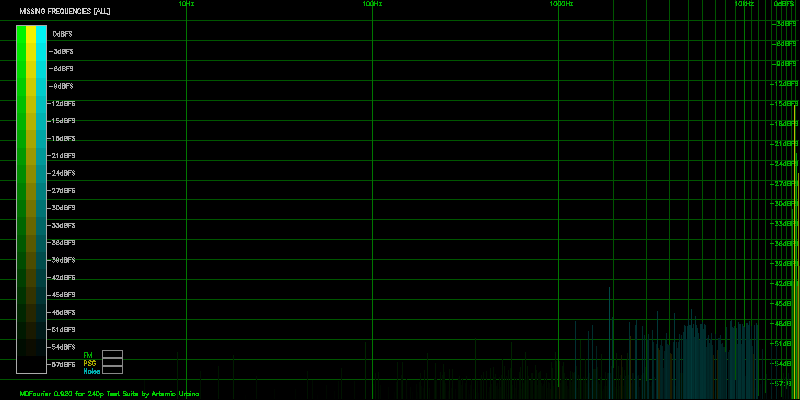
\includegraphics[width=1.0\linewidth]{images/interpretation/Plot6-mp3-3.png}
	\caption[MP3 Missing]{Missing frequencies from \ac{mp3}.}
	\label{fig:plot6-mp3-3}
\end{figure}

It can be appreciated that the missing frequencies were detected after the \khz{18} line, aside from some harmonics below \db{-45}.

\chapter{Results from vintage retail hardware}
\label{results}

The following table lists all the hardware used to make the recordings for the graphs in this chapter. All systems had stock parts at the time of recording, no modifications and used original power supplies.\footnote{They were all connected to a PVM-5041Q--a 4" \textit{CRT}--via \textit{RGB}, although the \textit{CRT} was turned off while recording. Since \textit{video refresh} noise is a very isolated frequency range it is not filtered out for comparisons, however it is detected and reported by the software for several purposes.}. 

The \textit{MDFourier ID} value in the following table refers to the file name in the catalog\footnote{All the recordings are available from the \textit{downloads page} from the \textit{MDFourier} website. See appendix \ref{downloads}.}. 

\begin{center}
\scalebox{0.6}{
\begin{tabular}{ | l | l | l | l | l | l | l | l | l | }
    \hline
	Type    & Model    & Revision & FCCID & Serial & Region & Made in & MDFourier ID & Recorded from\\
    \hline
	Model 1 & HAA-2510 & VA1    &               & 89N61751  & Japan & Japan  & A-MD1JJVA1   & Headphone Out\\
	Model 1 & 1601     & VA3    & FJ846EUSASEGA & 30W59853  & USA   & Taiwan & A-MD1UTVA3   & Headphone Out\\
	Model 1 & 1601     & VA3    & FJ846EUSASEGA & 30W59853  & USA   & Taiwan & A-MD1UTVA3-AV&  AV Out\\
	Model 1 & 1601     & VA6    & FJ8USASEGA    & B10120356 & USA   & Japan  & A-MD1UJVA6   & Headphone Out\\
	Model 1 & 1601     & VA6    & FJ8USASEGA    & 59006160  & USA	& Taiwan & A-MD1UTVA6-1 & Headphone Out\\
	Model 1 & 1601     & VA6    & FJ8USASEGA    & 31X73999  & USA   & Taiwan & A-MD1UTVA6-2 & Headphone Out\\
	Model 1 & HAA-2510 & VA6    &               & A10416197 & Japan	& Japan  & A-MD1JJVA6   & Headphone Out\\
	Model 2 & MK-1631  & VA1.8  & FJ8MD2SEGA    & 151014280 & USA   & China  & A-MD2UCVA18  & AV Out\\
	Nomad   & MK-6100  &        & 50059282	    &           & USA	& Taiwan & A-NMUT-AV    & AV Out\\
	Nomad   & MK-6100  &        & 50059282	    &           & USA	& Taiwan & A-NMUT       & Headphone Out\\
	CDX     & MK-4121  &        & Y40 014198    &           & USA   & Japan  & A-CDXUJ-LO   & Line Out\\
	CDX     & MK-4121  &        & Y40 014198    &           & USA   & Japan  & A-CDXUJ-HP   & Headphone Out\\
	CDX     & MK-4121  &        & Y40 014198    &           & USA   & Japan  & A-CDXUJ-AV   & AV Out\\
	\hline
\end{tabular}
}
\end{center}

It must be considered that this is a very small sample size, and no results or interpretations should be extrapolated as generalized conclusions about differences between models. 

However, since several common trends are found and the systems were sourced from very different providers across a long period, it would be too high a coincidence for these results to be by pure chance. I expect that we--as a community--can grow a bigger data set of recordings, in order to make better assessments in the future\footnote{I've consider the viability of creating "averaged" system profiles in the future--using an extra tool yet to be developed--that could give us a generalized profile created from multiple samples.}.

For simplicity, the recordings used were made with the \textit{USB Lexicon Alpha} audio card\footnote{Reasons are: flat frequency response, available in the market at the time of writing, works externally via USB and is not expensive. See appendix \ref{audiocards}.}. The first system is the \textit{Reference}, and the second one is the \textit{Comparison} signal.

Even if the system volume settings won't affect the analysis since \textit{normalization} is performed in software\footnote{For details in the \textit{normalization} procedures used, see appendix \ref{normalization}.}, the volume control was set to its maximum when using the \textit{headphone out} port. This was made in order to get consistent results, since variations could arise from the performance of the system amplifiers.

\section{Sega Genesis Model 1 VA3 (US) vs\\ Mega Drive Model 1 VA1 (JP)}

These models are an interesting starting point since the \textit{Reference} system--the \textit{VA3}\footnote{This refers to the motherboard revision in the system, see \cite{genesisaudio}.}--is usually considered\footnote{See \cite{genesisaudio2} for more information.} one of the best sounding versions of the system family line. 

On the other hand, the Japanese \textit{VA1} is the first revision to the launch \textit{JP VA0} system. This will give us an idea of how much the audio signatures changed from the launch units in Japan to the \textit{US VA3}--which is also the first revision to the USA system, where the launch unit was the \textit{VA2}\footnote{See \cite{genesishw} for information on hardware revisions.}.

\begin{figure}[H]
	\centering
	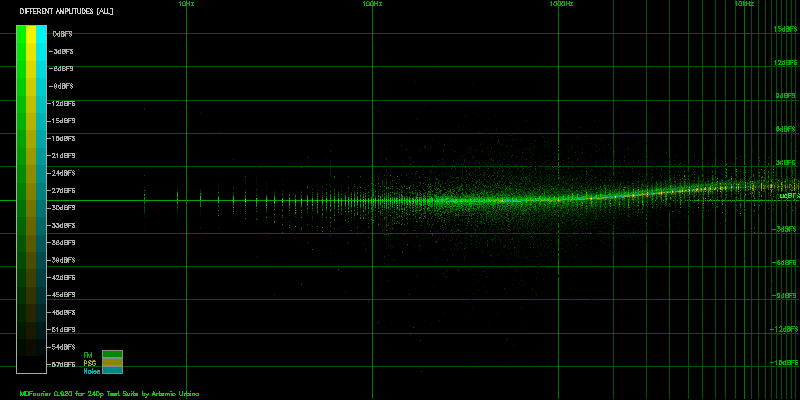
\includegraphics[width=1.0\linewidth]{images/results/1-A-MD1UTVA3-LA_vs_A-MD1JJVA1-LA.png}
	\caption[A-MD1UTVA3-LA vs A-MD1JJVA1-LA]{Differences between A-MD1UTVA3-LA and A-MD1JJVA1-LA.}
	\label{fig:A-MD1UTVA3-LA_vs_A-MD1JJVA1-LA}
\end{figure}

The resulting graph shows that the signals are quite similar, where only the higher frequencies--the treble--exhibit some deviation. The curve starts around \khz{2} and slowly rises about \db{1} above the \db{0} line.

It is generally accepted that the minimum perceivable difference--under normal conditions--is around \textit{3dB}\footnote{Under ideal conditions \textit{1dB} can be achieved, see \cite{dbdiff}.}. So although a measurable difference exists--which is possibly noticeable under ideal listening conditions--the systems are very similar.

It is also noticeable that the percentage match bars are full, meaning that practically all the frequencies compared were matched.

\section{Sega Genesis Model 1 VA3 (US):\\ Headphone out vs AV out}

Ever wondered if something was lost--besides stereo--when using the \textit{AV out} port from the console instead of the \textit{headphone out}? Figure \ref{fig:A-MD1UTVA3-LA_vs_A-MD1UTVA3-AV-LA} shows both ports compared using the same system.

\begin{figure}[H]
	\centering
	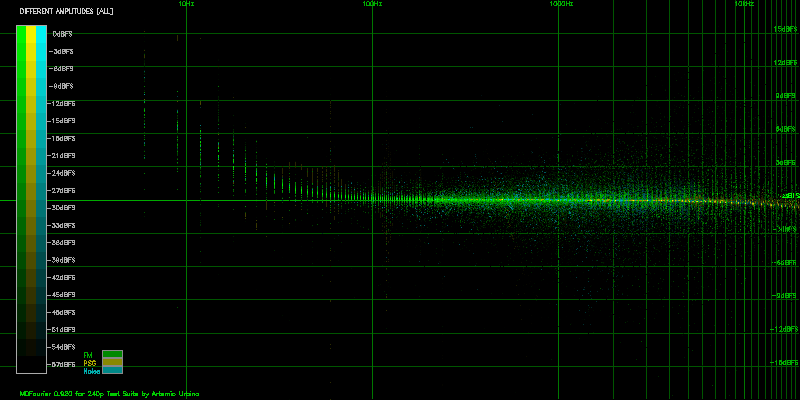
\includegraphics[width=1.0\linewidth]{images/results/1-A-MD1UTVA3-LA_vs_A-MD1UTVA3-AV-LA.png}
	\caption[A-MD1UTVA3-LA AV Out]{Differences between \textit{Headphone out} and \textit{AV out} for the A-MD1UTVA3-LA.}
	\label{fig:A-MD1UTVA3-LA_vs_A-MD1UTVA3-AV-LA}
\end{figure}

Differences are present only in \textit{bass}\footnote{Low frequency tones.} and \textit{treble}\footnote{high frequency tones.}. In the higher end of the spectrum, differences are less than \db{1} and higher than \khz{17}. The low end differences are more interesting--but still at a frequency range that would hardly matter for most setups, aside from the lost stereo. These reach a \db{3} difference around \hz{30}, so you get deeper bass when using the \textit{AV out} if the music\footnote{Yes, \textit{Bare Knuckle/Streets of Rage} does reach this part of the spectrum. It must be noted that most of the bass range is really between \hz{60}-\hz{500}. See \cite{bass}.} reaches those notes and your audio system has the means to reproduce it.

\section{Sega Genesis Model 1 VA3 (US) vs\\ Sega Genesis Model 1 VA6 (JP)}

We'll again be using the \textit{US VA3} as \textit{reference}, now contrasted against a \textit{Japanese VA6}. The \textit{VA6} is regarded as a good sounding unit in par with the \textit{VA3}\footnote{See \cite{genesisaudio} for details.}, and is also very common. 

\begin{figure}[H]
	\centering
	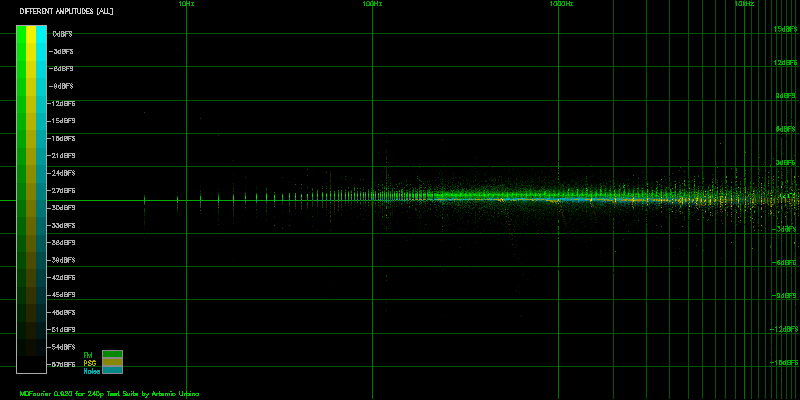
\includegraphics[width=1.0\linewidth]{images/results/2-A-MD1UTVA3-LA_vs_A-MD1JJVA6-LA.png}
	\caption[A-MD1UTVA3-LA vs A-MD1JJVA6-LA]{Differences between A-MD1UTVA3-LA and MD1JJVA6-LA.}
	\label{fig:A-MD1UTVA3-LA_vs_A-MD1JJVA6-LA}
\end{figure}

The curves closely follow the \db{0} line, however the \textit{YM2612}\footnote{The \textit{Yamaha 2612} synthesizer--also known as \textit{YM2612}--is responsible for the \textit{FM} sound in this systems.} amplitude is higher than the \textit{PSG} amplitude by a really low margin, around \db{0.4}. Although measurable, this would be even less noticeable than the difference against the \textit{VA1}.

\section{Sega Genesis Model 1 VA6 (JP) vs\\ Mega Drive Model 1 VA6 (US)}

We'll now compare two systems with the same \textit{VA6} motherboard revision. However, one is Japanese and the other is from North America. Results are displayed in Figure \ref{fig:A-MD1JJVA6-LA_vs_A-MD1UJVA6-LA}.

\begin{figure}[H]
	\centering
	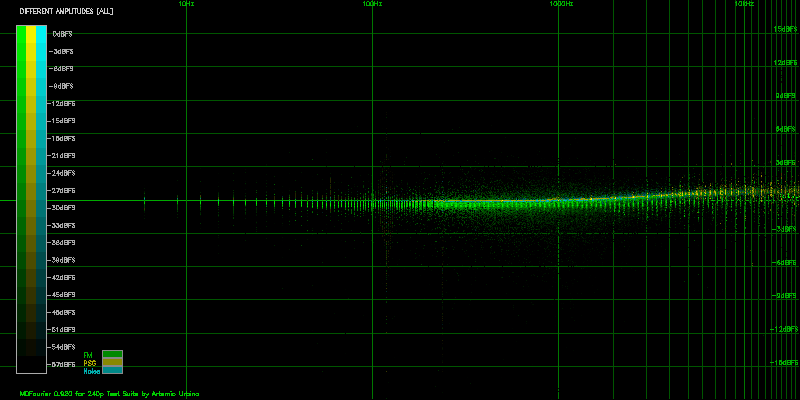
\includegraphics[width=1.0\linewidth]{images/results/3-A-MD1JJVA6-LA_vs_A-MD1UJVA6-LA.png}
	\caption[A-MD1JJVA6-LA vs A-MD1UJVA6-LA]{Differences between A-MD1JJVA6-LA and A-MD1UJVA6-LA.}
	\label{fig:A-MD1JJVA6-LA_vs_A-MD1UJVA6-LA}
\end{figure}

Once again, differences are minimal and quite similar to some previous results--in particular to the ones between the \textit{US VA3} and the \textit{JP VA1}. But now \textit{FM} seems to be closer and \textit{PSG} is the one that is less than \db{1} higher on the \textit{US} system.

\section{Sega Genesis Model 1 VA6 (US) vs\\ Sega Genesis Model 1 VA6 (US)}

These are two other \textit{US VA6} systems, both made in \textit{Taiwan}. And here are the results:

\begin{figure}[H]
	\centering
	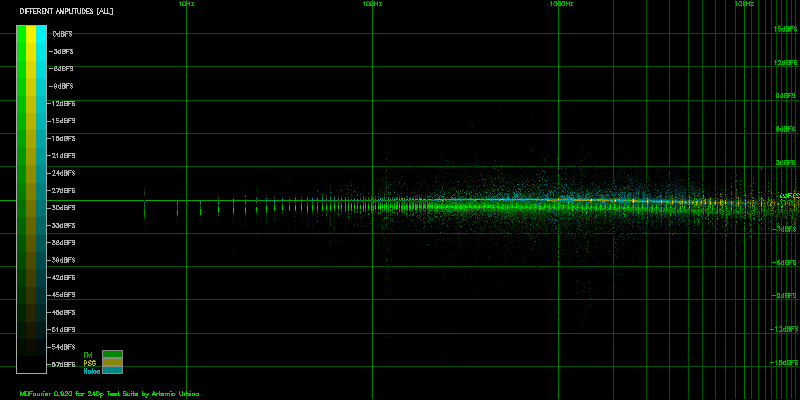
\includegraphics[width=1.0\linewidth]{images/results/4-A-MD1UTVA6-1-LA_vs_A-MD1UTVA6-2-LA.png}
	\caption[A-MD1UTVA6-1-LA vs A-MD1UTVA6-2-LA]{Differences between A-MD1UTVA6-1-LA and A-MD1UTVA6-2-LA.}
	\label{fig:A-MD1UTVA6-1-LA_vs_A-MD1UTVA6-2-LA}
\end{figure}

Again, these are very close matches with differences below \db{1}. In this case \textit{FM} is lower by that amount and \textit{PSG} matches the reference unit.

\section{Sega Genesis Model 1 VA3 (US) vs\\ Sega Genesis Model 2 VA1.8 (US)}

And now for something a bit more interesting. The same American \textit{VA3} unit we've compared to a few others, but contrasted against a \textit{Model 2 VA1.8}. These \textit{Model 2} systems don't use the \textit{YM2612}, but an \define{asic} \textit{Yamaha YM3438}, which is a variation used for some later models.

These \textit{Model 2} versions--grouped with \textit{VA7} and other revisions--are regarded as having a lower quality sound output. This is due to various factors: the variation in \textit{FM} synthesizer, the amplifier circuits used and the general audio circuit design.

\begin{figure}[H]
	\centering
	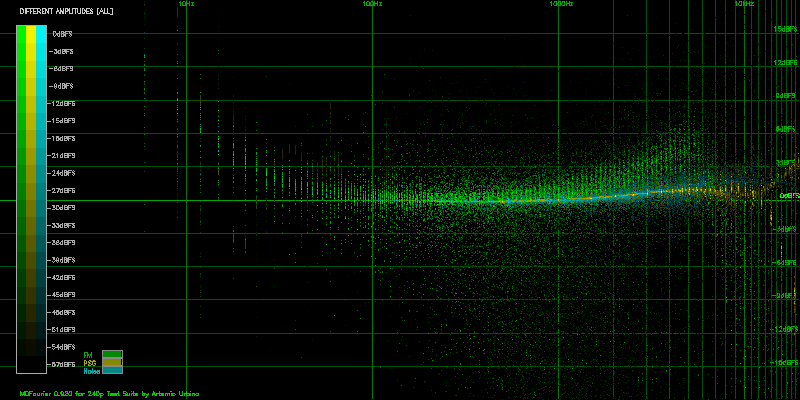
\includegraphics[width=1.0\linewidth]{images/results/5-1-A-MD1UTVA3-LA_vs_A-MD2UCVA18-LA.png}
	\caption[A-MD1UTVA3-LA vs A-MD2UCVA18-LA]{Differences between A-MD1UTVA3-LA and A-MD2UCVA18-LA.}
	\label{fig:A-MD1UTVA3-LA_vs_A-MD2UCVA18-LA}
\end{figure}

The differences in this case are more noticeable: \textit{FM} raises above \db{3}--which is generally accepted as a discernible threshold\footnote{See \cite{dbdiff} for results from different studies.}--and does this around frequencies to which our hearing is quite sensitive\footnote{Since this range falls within the spectrum for human voice, see \cite{humanvoice}.}, from \khz{2} to around \khz{8}.

But since a lot of data points are highly scattered, we can gather more accurate information for analysis using the \textit{Average Graph} option as shown in Figure \ref{fig:A-MD1UTVA3-LA_vs_A-MD2UCVA18-LA_AVG}.

\begin{figure}[H]
	\centering
	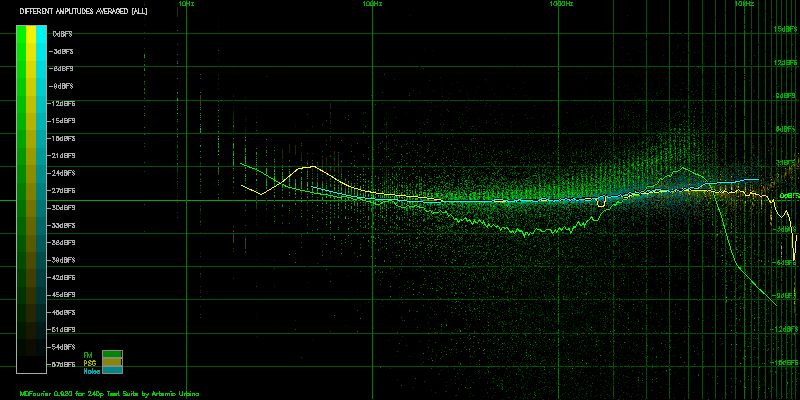
\includegraphics[width=1.0\linewidth]{images/results/5-2-A-MD1UTVA3-LA_vs_A-MD2UCVA18-LA.png}
	\caption[A-MD1UTVA3-LA vs A-MD2UCVA18-LA Averaged]{Averaged Differences between A-MD1UTVA3-LA and A-MD2UCVA18-LA.}
	\label{fig:A-MD1UTVA3-LA_vs_A-MD2UCVA18-LA_AVG}
\end{figure}

We can now appreciate that there are some relevant frequencies--that is, \textit{high amplitude} in the \textit{reference} signal--that pull the averaged graph lower between \hz{200} and \khz{3}-\textit{FM} spectrum, and these go down up to \db{3}.

We can also make out that peak in the human voice spectrum that goes \db{3} higher, and then it dips in the treble above \khz{6} to amplitudes lower by \db{6} after \khz{10}.

On the other hand, \textit{PSG} seems quite similar aside from a bump around \hz{60} and dipping in amplitude after \khz{14}.

It must also be noted that, for the first time, there is a drop in the percentage of matched frequencies, shown in the bars detailed in Figure \ref{fig:A-MD1UTVA3-LA_vs_A-MD2UCVA18-LA_BARS}.

\begin{figure}[H]
	\centering
	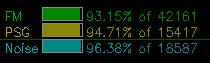
\includegraphics[width=0.4\linewidth]{images/results/5-3-A-MD1UTVA3-LA_vs_A-MD2UCVA18-LA_bars.png}
	\caption[A-MD1UTVA3-LA vs A-MD2UCVA18-LA Bars]{Percentage Match Bars between A-MD1UTVA3-LA and A-MD2UCVA18-LA.}
	\label{fig:A-MD1UTVA3-LA_vs_A-MD2UCVA18-LA_BARS}
\end{figure}

So far we had been getting results above \textit{99.7\%}, and this time it droped to \textit{93.15\%} for \textit{FM}.

\section{Sega Genesis Model 1 VA3 (US) vs\\ Sega Nomad (US)}

The \textit{Sega Nomad} is a portable version of the \textit{Sega Genesis}, and it had only a single motherboard revision. Recordings were made via both: \textit{AV out} and \textit{headphone out}. 

Our first contrast example will be using the \textit{headphone out} port from both consoles, shown in Figure \ref{fig:A-MD1UTVA3-LA_vs_A-NMUT-LA}.

\begin{figure}[H]
	\centering
	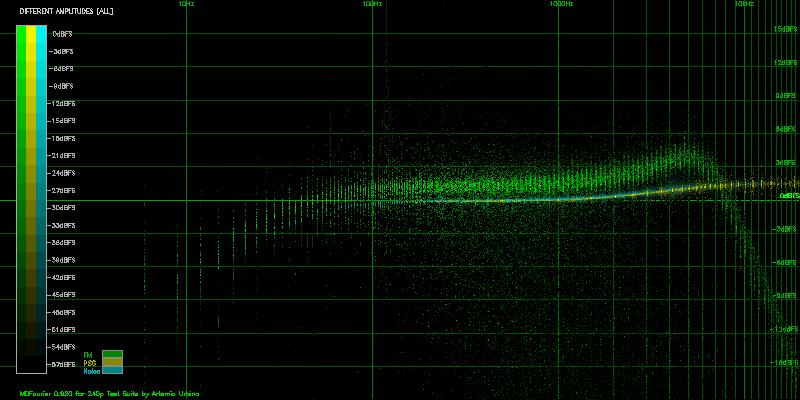
\includegraphics[width=1.0\linewidth]{images/results/6-A-MD1UTVA3-LA_vs_A-NMUT-LA.png}
	\caption[A-MD1UTVA3-LA vs A-NMUT-LA]{Differences between A-MD1UTVA3-LA and A-NMUT-LA.}
	\label{fig:A-MD1UTVA3-LA_vs_A-NMUT-LA}
\end{figure}

Some resemblance to the previous comparison to the \textit{Model 2 VA1.8} can be seen. In order to contrast both signals, an \textit{averaged graph} is shown below.

\begin{figure}[H]
	\centering
	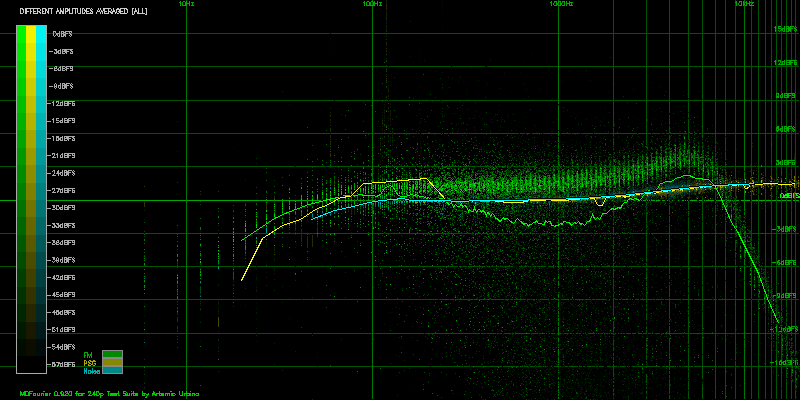
\includegraphics[width=1.0\linewidth]{images/results/6-A-MD1UTVA3-LA_vs_A-NMUT-LA-AVG.png}
	\caption[A-MD1UTVA3-LA vs A-NMUT-LA AVG]{Averaged Differences between A-MD1UTVA3-LA and A-NMUT-LA.}
	\label{fig:A-MD1UTVA3-LA_vs_A-NMUT-LA_AVG}
\end{figure}

The same general behavior from figure \ref{fig:A-MD1UTVA3-LA_vs_A-MD2UCVA18-LA_AVG} can be seen in \textit{FM}, but \textit{PSG} doesn't fall in the same way in the high frequency range. This must be due to differences in the \textit{mixing circuit} or amplifiers.

And if you've wondered about the difference between using the headphone out or the AV out in a Sega Nomad, here are the results:

\begin{figure}[H]
	\centering
	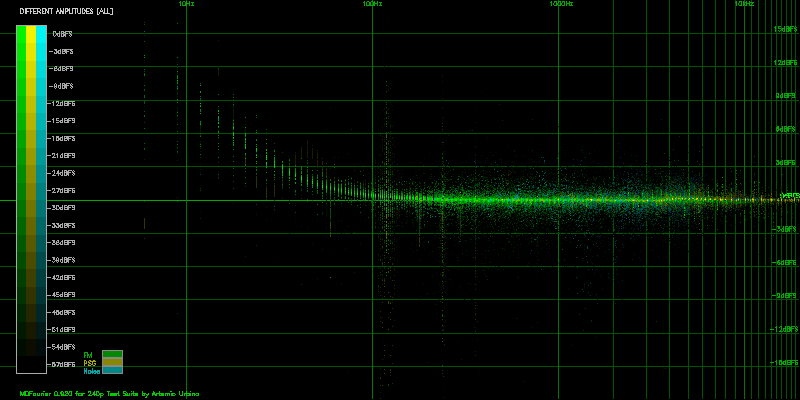
\includegraphics[width=1.0\linewidth]{images/results/6-A-NMUT-LA_vs_A-NMUT-AV-LA.png}
	\caption[A-NMUT-LA vs A-NMUT-AV-LA]{Sega Nomad: \textit{headphone} vs \textit{AV out}.}
	\label{fig:A-NMUT-LA_vs_A-NMUT-AV-LA}
\end{figure}

In this case there are no differences above \hz{100}. However the AV out has a more low frequency emphasis that is \db{3} higher below \hz{40}.

\section{Sega Genesis Model 2 VA1.8 (US) vs\\ Sega Nomad (US)}

Due to the similarities shown between the \textit{Nomad} and the \textit{Model 2 VA 1.8} when contrasted against the \textit{Model 1 VA3}, here is the comparison between them using the \textit{AV out}.

\begin{figure}[H]
	\centering
	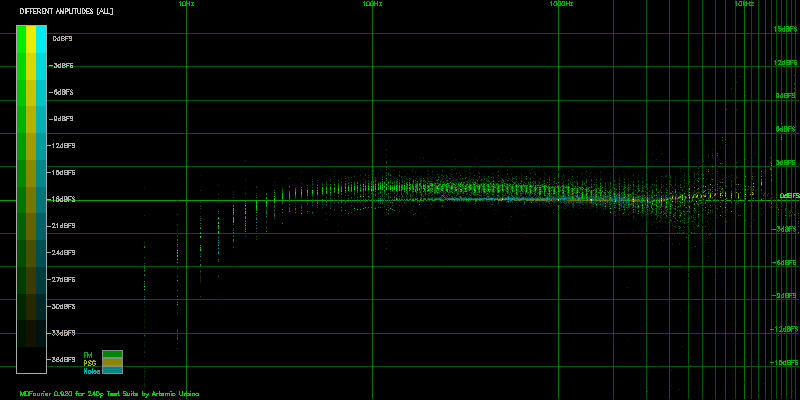
\includegraphics[width=1.0\linewidth]{images/results/7-A-MD2UCVA18-LA_vs_A-NMUT-LA.png}
	\caption[9-A-MD2UCVA18-LA vs A-NMUT-LA]{Differences between A-MD2UCVA18-LA vs A-NMUT-LA.}
	\label{fig:A-MD2UCVA18-LA_vs_A-NMUT-LA}
\end{figure}

The consoles are indeed similar between themselves, with differences probably arising from amplification circuits. The \textit{Low pass filter} is steeper in the \textit{Sega Nomad} for \textit{FM}, among other differences in the high rage regarding \textit{PSG}.

Another interesting point is that both of these systems exhibit video refresh noise at a higher amplitude via the \textit{AV out} than their \textit{Model 1} counterparts: around \db{-45} instead of \db{-70}.

\section{Sega Genesis Model 1 VA3 (US) vs\\ Sega CDX (US)}

The \textit{Sega CDX} is an all-in-one system that includes the \textit{Sega CD} unit. It has three different output options: \textit{headphone out}, \textit{line out} and \textit{AV out}.

We'll start by with the results of the \textit{Model 1} as \textit{reference} contrasted to the \textit{CDX line out}.

\begin{figure}[H]
	\centering
	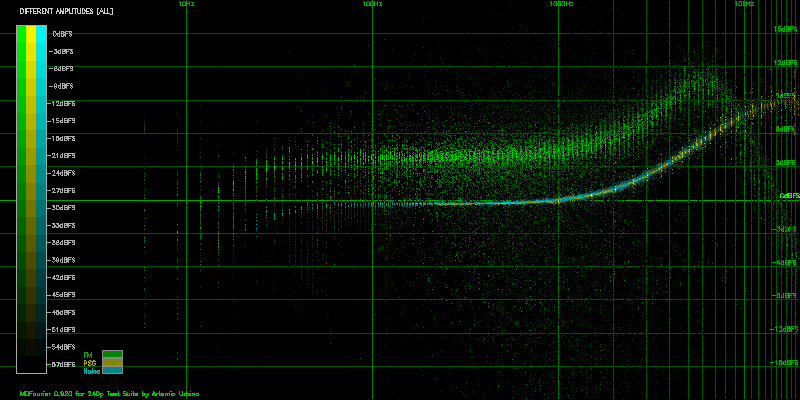
\includegraphics[width=1.0\linewidth]{images/results/8-A-MD1UTVA3-LA_vs_A-CDXUJ-LO-LA.png}
	\caption[A-MD1UTVA3-LA vs A-CDXUJ-LO-LA]{Differences between A-MD1UTVA3-LA and A-CDXUJ-LO-LA.}
	\label{fig:A-MD1UTVA3-LA_vs_A-CDXUJ-LO-LA}
\end{figure}

These are easily the most notorious differences between \textit{vintage retail hardware} I've found so far. 

The \textit{CDX PSG} does not have the low pass filter present in \textit{Model 1} systems. The \textit{FM} output is higher by at least \db{3}, and it has a \textit{low pass filer} around \khz{9}.

Figure \ref{fig:A-MD1UTVA3-LA_vs_A-CDXUJ-LO-LA_AVG} shows the results when the \textit{average} option is enabled.

\begin{figure}[H]
	\centering
	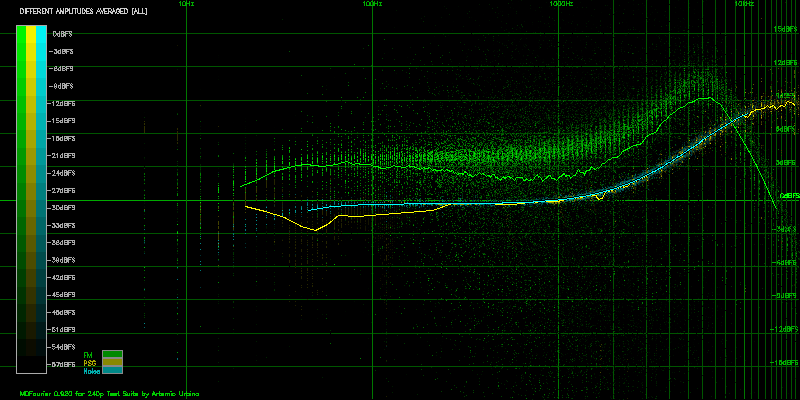
\includegraphics[width=1.0\linewidth]{images/results/8-A-MD1UTVA3-LA_vs_A-CDXUJ-LO-LA-avg.png}
	\caption[A-MD1UTVA3-LA vs A-CDXUJ-LO-LA AVG]{Differences between A-MD1UTVA3-LA and A-CDXUJ-LO-LA Averaged.}
	\label{fig:A-MD1UTVA3-LA_vs_A-CDXUJ-LO-LA_AVG}
\end{figure}

This makes it easier to discern the curve that the \textit{FM} audio follows when compared to the \textit{Model 1}. It reaches as up to \db{9} higher between the \khz{4}-\khz{9} range.

We must remember that the \textit{Model 1}, used here as reference, has it's highest amplitude in the PSG signal with the current test. That's why the results show FM higher instead of a lower \textit{PSG}, since \textit{MDFourier} does relative comparisons based on the \textit{Reference} signal.

\section{Sega CDX (US) Line-out vs\\ Sega CDX (US) Headphone port}

And for completeness, here is the \textit{differences} graph when contrasting the \textit{Sega CDX} \textit{line out} vs the \textit{headphone out}.

\begin{figure}[H]
	\centering
	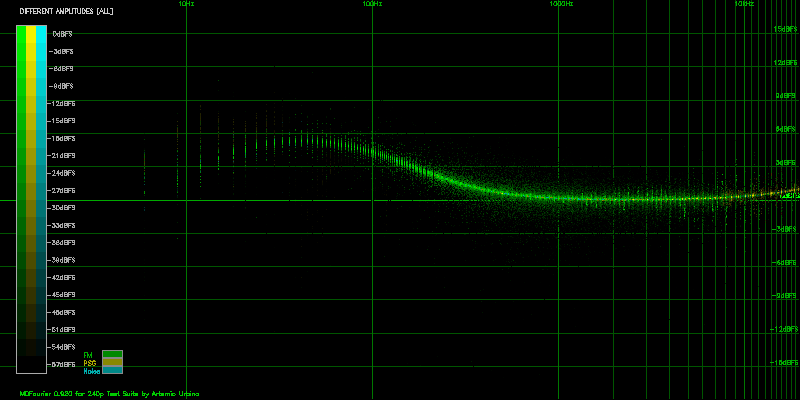
\includegraphics[width=1.0\linewidth]{images/results/9-A-CDXUJ-LO-LA_vs_A-CDXUJ-HP-LA.png}
	\caption[A-CDXUJ-LO-LA vs A-CDXUJ-HP-LA]{Differences between A-CDXUJ-LO-LA and A-CDXUJ-HP-LA.}
	\label{fig:A-CDXUJ-LO-LA_vs_A-CDXUJ-HP-LA}
\end{figure}

The \textit{headphone out} has clear emphasis in the low frequency range, and even below \khz{1.5}.

\chapter{Future developments}

\textit{PC Engine/Turbo Grafx-16} support would be the my next target, to be followed by all the platforms that are currently supported by the \textit{240p Test Suite}.

\chapter{Conclusions}

So far \textit{MDFourier} has shown results that are consistent with previous empirical evaluations, and can support many such claims with data. I hope it can provide the community with a process that is repeatable and objective that can be used in any project where someone wants to preserve, compare, replicate or play with the results.

I believe these cases support the idea that this process has value, and that it can be replicated in as many platforms as possible. Audio has been historically relegated to a secondary position, when the audio visual experience is one--as a whole. Games are not the same without their acoustic experience.

This could help to document the original audio signatures of old systems. And of course, to enable the community to play with variations and modifications that are as valid as the ones the systems originally had at launch.

\begin{appendices}
	
\chapter{Downloads}
\label{downloads}

The project web page is available at \url{http://junkerhq.net/MDFourier/}, where the latest version of this document is available in \textit{PDF} and \textit{HTML}.

The \textit{Downloads} page contains the following items:
\begin{itemize}
	\item A pre-compiled \textit{Microsoft Windows} executable of the latest build with \ac{gui} for the \textit{Analysis Software}.
	\item The \textit{Tone Generator} software for each supported platform.
	\item Updated source code for all tools.
	\item Sample recordings used for the creation of this document as detailed in chapter \ref{results}.
\end{itemize}
	
\chapter{How to use the \textit{Analysis Software}}
\label{usinggui}
The current version of the \textit{Analysis Software} allows access to the main options of \textit{MDFourier}. It is a \textit{Windows} executable and all corresponding files must be placed in the same folder. \textit{Uncompressing} the package to a folder should have all that is necessary to run the program.

After executing \textit{MDFourierGUI.exe} you should be presented with the following interface:

\begin{figure}[H]
	\centering
	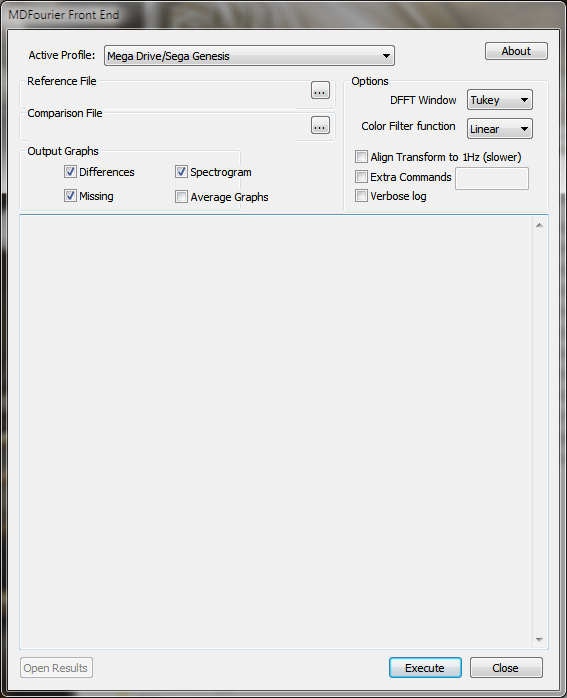
\includegraphics[width=0.6\linewidth]{images/GUI/GUI1.png}
	\caption[Front End]{\textit{MDFourier} Windows Front End for the \textit{Analysis Software}.}
	\label{fig:gui1}
\end{figure}

In order to generate the output graphs, two files must be selected to compare them. One as a \textit{Reference} and the other as the \textit{Comparison} file, as detailed in section \ref{workflow}.

The following sequence of steps indicates the typical work flow within the \ac{gui}:

\begin{figure}[H]
	\centering
	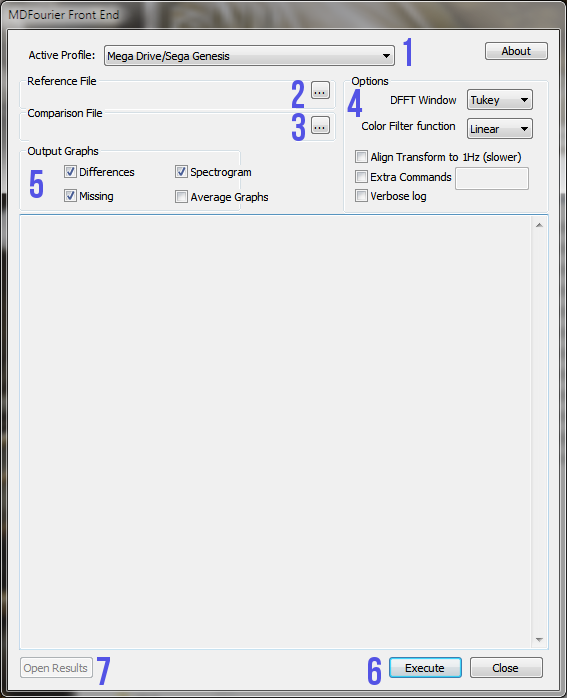
\includegraphics[width=0.6\linewidth]{images/GUI/GUI2.png}
	\caption[Steps]{Typical sequence of steps.}
	\label{fig:gui2}
\end{figure}

\begin{enumerate}
	\item Select a \textit{Profile} for the analysis.
	\item Select a \textit{Reference} file.
	\item Select a \textit{Comparison} file.
	\item Change the default \textit{options} if needed.
	\item Select the desired output \textit{graphs}.
	\item Execute \textit{MDFourier}.
	\item When execution ends, open the \textit{results folder}.
\end{enumerate}

The \textit{Analysis Software} will display the output text from the command line tool, including any errors or progress as it becomes available.

Keep in mind that the \textit{Open Results} button will only be enabled after a successful comparison between files has finished, and it won't open a second instance of the window if you have one already present.

The default options will generate graphs that work on most situations. In some cases fine tuning the results might highlight specific aspects. These options will be described in the following sections.

\section{Analysis Tool Options}

The currently available options in the \textit{Analysis Software} are:

\subsection{Window Functions}
\label{windows}

In order to reduce \textit{spectral leakage}\footnote{This term describes new frequency components created when applying a Fourier Transform to a segment of a signal. See \cite{leakage}.} when applying the \ac{dft}, a \textit{filtering window}\footnote{All details regarding the windows used, their formulas and graphs are in appendix \ref{windowfunctiondetails}.} is applied to each element to be compared between both signals. Since we are producing the sound ourselves from the \textit{Tone Generator}, the signal can be analyzed as \textit{periodic}\footnote{In theory this means we could get away without applying a window, but in practice the signal is not perfect and \textit{windowing} the data helps to eliminate noise.}, and has a natural \textit{attack} and \textit{decay} rate if possible.

By default we use a custom \textit{Tukey window}\footnote{This is not a common choice for window function, but was selected due to the above reasons after comparing results with  the rest of the available options.} with very steep slopes. \textit{MDFourier} does offer alternate windows as options for further analysis.

\subsection{Color Filter Functions}
\label{colorfilter}

Each dot in the \textit{Differences} graph uses the \textit{X axis} for the frequency range and the \textit{Y axis} for the amplitude difference between the \textit{Comparison} and \textit{Reference} signals.\footnote{See section \ref{outputfiles} for output file details.}

Color intensity of each dot is used to represent the amplitude for that frequency in the \textit{Reference} signal. In other words, how relevant it was to create the original signal in that note. Please refer to chapter \ref{howtographs} in order to see examples of their use.

A color scale is presented in each graph, with the color graduation and the corresponding amplitude level.

\begin{figure}[H]
	\centering
	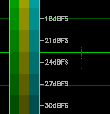
\includegraphics[width=0.2\linewidth]{images/colorfilter/colorscale.png}
	\caption[Graph color scale]{Detail of color scale in graph.}
	\label{fig:colorscale}
\end{figure}

The options are useful to \textit{highlight} or \textit{attenuate} these differences by applying the range to one of the following functions. 

They are sorted in descending order. The topmost option will highlight all differences; and the bottom one will attenuate most of them, and show just the ones with highest amplitudes in the \textit{Reference} signal.

All filters, their graphs and effects are listed in appendix \ref{filterfunctions}.

\subsection{Align Transform to 1Hz}

When designing the \textit{audio signal} for use during analysis, one consideration is how to balance gathering more information versus the duration of each recording. 

For practical reasons, it is desirable to have a short test that will be recorded for analysis. This reduces the time it takes to digitize audio from several systems, the storage used, analysis time by the software, and makes distributing such files easier.

In contrast, when applying the \textit{Fourier transform} a compromise is made between frequency detail and time accuracy, very similar to the Heisenberg's uncertainty principle. If we compare a longer signal for each element, we end up with more frequency information. In our case, we don't care much about time accuracy but we do care about the length of the test. Nobody wants to record a 5 or 10 minute signal for each test to be made.

The compromise made is to use \textit{sub second signals} for each element to be compared. Since the time and sample rate determine how the \ac{dft} \textit{frequency bins}\footnote{The size of each slice in \acrlong{hz} for the frequency spectrum.} are spaced after analysis--and how much information we end up analyzing--the end result is a lower graph resolution.

Zero padding the input signal for Fourier analysis is a controversial subject\footnote{Zero-padding a signal does not reveal more information about the spectrum. See \cite{zeropaddinginterpolate} \cite{ZeroPaddingBad}.}, but for the present application no adverse effects have been found. This might be the case since we control how the source signal is generated, with a predetermined \textit{attack} and \textit{decay}. However, it is disabled by default so the results presented can be free from questioning regarding the effects, and available for cases where more precise frequency information is needed with no spectral leakage to adjacent \textit{frequency bins}.

\subsection{Output Graphs}
\label{outputfiles}

Several graphs will be generated as a result of the analysis. There will be several graphs of each type in the \textit{output folder}\footnote{It is named \textit{MDFourier} and a subfolder named as the compared files. It can be accessed from the \textit{Analysis Software} with the \textit{Open Results} button.}. One for each type, and one that summarizes all types in a single graph.

All graphs are saved in the \defineCite{png}{support via \textit{libpng} \cite{libpng}} format, which is lossless and open source. Please read section \ref{howtographs} for examples and a guide to interpret their meaning. 

\subsubsection{Different Amplitudes}

Enabling this option creates the most relevant output graphs from \textit{MDFouriuer}. These contain the amplitude difference for the frequencies common to both files across the hearing spectrum using the \textit{Reference} file as control.

If the files are identical, the graph will be a perfect line across the \db{0} line. In case the signals differ, a scatter graph will show how it behaves across the typical human hearing spectrum\footnote{Typically defined as \hz{20-20000}, but the higher end tends to be lost with age.}.

The file names for these graphs have the format:\\ \textit{DA\_Reference\_vs\_Comparison\_block\_options.png}

\subsubsection{Missing Frequencies} 

Graphs the frequencies available in the \textit{Reference} file but not found in the \textit{Comparison} file within the significant amplitude range. This is in effect a \textit{Spectrogram}, but limited to the frequencies that were expected to be in the intersection but that were not present in the \textit{Comparison} file.

The file names for these graphs have the format:\\ \textit{MIS\_Reference\_vs\_Comparison\_block\_options.png}

\subsubsection{Average Graphs}
\label{averaged}

This option traces an \textit{average line} on top of the \textit{Difference} graphs, making it easier to follow the trend when the output has severely scattered data. It is \textit{off by default}.

The curve is created by averaging time segments from the frequency data sorted in ascending order. A \textit{Simple Moving Average}\footnote{This is a type of average that is intended to smooth out sudden peaks in the data. Often used in exchange rate graphs. See \cite{sma}.} is then calculated to smooth out the results.

The curve is weighted according to the \textit{Color Filter Functions} described in section \ref{colorfilter}, by repeating each data point by the amount mapped in the \textit{0-1} interval described by the function.

As a result, the average will follow the relative amplitudes from the \textit{Reference} signal proportional to the selected \textit{filter function}.

If there is need for a graph without weighting, please disable the \textit{Color Filtering function}.

The file names for these graphs have the format:\\ \textit{DA\_AVG\_Reference\_vs\_Comparison\_block\_options.png}

\subsubsection{Spectrograms}

Plots all the frequencies available in each file\footnote{As limited by the analysis parameters, such as amplitude and frequency count per block.}. Two sets of spectrograms are generated, one for the \textit{Reference} file and one for the \textit{Comparison} file.

The file names for these graphs have the format:\\ \textit{SP\_AVG\_Reference\_vs\_Comparison\_block\_options.png}

\subsection{Extra Command}
\label{extracommand}

This checkbox enables the text field to send any extra commands that are not available via the \ac{gui} to \textit{MDFourier}. 

Current options as of version \textit{0.918} are:

\begin{verbatim}
MDFourier 0.918 [240p Test Suite Fourier Audio compare tool]
Artemio Urbina 2019 free software under GPL

usage: mdfourier -r reference.wav -c compare.wav
FFT and Analysis options:
-a: select <a>udio channel to compare. 's', 'l' or 'r'
-w: enable <w>indowing. Default is a custom Tukey window.
'n' none, 't' Tukey, 'h' Hann, 'f' FlatTop & 'm' Hamming
-f: Change the number of analyzed frequencies to use from FFTW
-s: Defines <s>tart of the frequency range to compare with FFT
-e: Defines <e>nd of the frequency range to compare with FFT
-i: <i>gnores the silence block noise floor if present
-t: Defines the <t>olerance when comparing amplitudes in dBFS
-z: Uses <z>ero Padding to equal 1 hz FFT bins
-n: <N>ormalize: 't' Time Domain Max, 'f' Frequency Domain Max or 'a' Average
-B: Do not do stereo channel audio <B>alancing
Output options:
-l: <l>og output to file [reference]_vs_[compare].txt
-v: Enable <v>erbose mode, spits all the FFTW results
-g: Create avera<g>e points over the plotted graphs
-A: Do not weight values in <A>veraged Plot (implies -g)
-L: Create 800x400 plots as shown in the manual
-H: Create 1920x1080 plots
-D: Don't create <D>ifferences Plots
-M: Don't create <M>issing Plots
-S: Don't create <S>pectrogram Plots
-d: Max <d>BFS for plots vertically
-k: cloc<k> FFTW operations
-j: (text) Cuts per block information and shows <j>ust total results
-x: (text) Enables e<x>tended log results. Shows a table with all matches
-m: (text) Enables Show all blocks compared with <m>atched frequencies
-h: Shows command line help
\end{verbatim}

Sending \textit{-h} in this field will enlist all the currently supported options for your version.

\subsection{Verbose Log}
\label{verbose}

A log is always created by default when using the \textit{Font End}, however this option enables a verbose version with the whole frequency analysis and many other details dumped to the file. 

Useful for reporting errors or unexpected behavior. \textit{Please send the audio files if possible as well!}\footnote{Contact details are available in appendix \ref{contact}.}
	
\chapter{Configuration file}
\label{mfnconfig}

All these parameters are defined in the \textit{mfn} configuration files inside the \textit{profiles} folder.\footnote{Different profiles can be used and selected via the \textit{Analysis Software}. There is one profile for each supported hardware platform.}. Here is the profile used to compare \textit{Mega Drive/Genesis} audio characteristics:

\begin{verbatim}
MDFourierAudioBlockFile 1.0
MegaDriveAudio
16.688
8820 -25 25 14 18 10
7
Sync s 1 20 red s
Silence n 1 20 red s
FM 1 96 20 green s
PSG 2 60 20 yellow m
Noise 3 16 20 aqua m
Silence n 1 20 red s
Sync s 1 20 red s
\end{verbatim}

This file defines what \textit{MDFourier} must do and how to interpret the \ac{wav} files. For now it can read \khz{44.1} and \khz{48} files, in Stereo \ac{pcm} format.

The first line is just a header, so that the program knows it is a valid file and in the current format.

The second line is the name of the current configuration, since I plan to add support for different consoles or arcade hardware in the future. This would imply creating a new \textit{mfn} file for each configuration, and a specific \textit{Tone Generator} to be run on the hardware.

The third line is the expected \textit{frame rate}\footnote{For more details regarding frame rate, see appendix \ref{framerate}.}. This is only used as a reference to estimate the placement for the blocks within the file before calculating the precise \textit{frame rate} of the recording as captured by the \textit{sound card}. After that is calculated, each signal uses its own timing in order to be fully aligned. \textit{Frame rate} variations in the order of \textit{0.001}\ac{ms} are natural, since we have an error of $\sfrac{1}{4}$ of a millisecond\footnote{For reference $\sfrac{1}{4}$ of a millisecond corresponds to 0.00025 seconds. Modern systems have different frame rates adapted for modern displays, small differences are more likely caused by the audio capture hardware \cite{SoundCardClock}.} during alignment, and differences also occur by the deviations in \textit{sample rates} and audio card limitations\footnote{See appendix \ref{audiocards}.}.

The fourth line defines the characteristics of the pulse tone used to identify the starting and end points of the signal within the \ac{wav} file. Its frequency, relative \textit{amplitude difference} to the \textit{background noise} (silence), and length \textit{intervals} that will be better explained in future revisions of this document.

The fifth line defines how many different blocks are to be identified within the files. There are seven blocks in this case.

Each block is composed of six characteristics: A \textit{Name}, a \textit{type}, the \textit{total number of elements} that compose it, the \textit{duration} for each element specified in frames, the \textit{color}\footnote{Available colors are listed in Appendix \ref{availablecolors}.} to be used for identifying it when plotting the results and a letter marking if it is a \textit{stereo} or \textit{mono} element\footnote{This is important for stereo audio balancing, see appendix \ref{stereobalancing}.}. Each block must correspond to a line with these parameters.

For example, FM audio has been named \textit{"FM"}, type \textit{1}, \textit{96} elements of \textit{20} frames each and will be colored in \textit{green}. Definition is in frames since emulators and \ac{fpga} implementations tend to run at different frame rates than the vintage retail platform, which result in different durations. The only way to align them, is by respecting the driving force that tied this up in the old days: the video signal.

There are currently two special types, identified by the letters \textit{'s'} and \textit{'n'}. The first one defines a \textit{sync pulse}, which is used to automatically recognize the starting and ending points of the signal inside the \ac{wav} file. 

The second one is for null audio, or silence. This \textit{silence} is used to measure the \textit{background noise}\footnote{How analysis is affected by this is described in section \ref{MinSigAmplitude}.} as recorded by the audio card. 	

\chapter{MDWave}
\label{mdwave}

\textit{MDWave} is a companion command line tool to \textit{MDFourier}. During development and while learning about \textit{DSP}, I needed to check what I was doing in a more tangible way. So, in order to visualize the files in an audio editor and listen to the results \textit{MDWave} was born.

It takes a single \ac{wav} file as argument, and loads all the parameters defined in the configuration file in order to verify the same environment\footnote{See appendix \ref{mfnconfig}.}.

The output is stored under the folder \textit{MDWave}, and a subfolder with the name of the input audio file. The default output is a \ac{wav} file named \textit{Used} which has the reconstructed signal from the original file after removing all frequencies that were discarded by the parameters used.

This means that it does a \textit{Fourier Transform}, applies the selected \textit{window}\footnote{See appendix \ref{windows}.} and estimates the noise floor. The highest amplitude frequencies are identified and limited by range for each element defined in the configuration file, and rest are discarded. An \textit{Inverse Fourier Transform} is applied in order to reconstruct the \ac{wav} file and the results are saved.

The opposite can be done as well by specifying the \textit{-x} option, and the result is a \textit{Discarded} \ac{wav} file, that has all the audio information that was deemed irrelevant and discarded by the specified options. With this you can listen to these and determine if a more severe comparison is needed.

In addition, the \textit{-c} option creates a \ac{wav} file with the chunk that corresponds to each element from the \textit{Reference} file being used, trimmed using the detected frame rate. Two chunks are created for each element, the \textit{Source} \ac{wav} chunk has the element trimmed without modification and the \textit{Processed} \ac{wav} chunk has the same element but with the windows and frequency trimming applied.

It has a few more command line options, which I'll detail in later revisions of the document. You can type \textit{mdwave -h} in your \textit{mdfourier} folder for details.

\begin{verbatim}
MDWave 0.920 (MDFourier Companion)
[240p Test Suite Fourier Audio compare tool]
Artemio Urbina 2019 free software under GPL

usage: mdwave -r reference.wav
FFT and Analysis options:
-a: select <a>udio channel to compare. 's', 'l' or 'r'
-c: Enable Audio <c>hunk creation, an individual WAV for each block
-w: enable <w>indowing. Default is a custom Tukey window.
'n' none, 't' Tukey, 'h' Hann, 'f' FlatTop & 'm' Hamming
-x: e<x>cludes results to generate discarded frequencies wav file
-i: <i>gnores the silence block noise floor if present
-f: Change the number of <f>requencies to use from FFTW
-s: Defines <s>tart of the frequency range to compare with FFT
-e: Defines <e>nd of the frequency range to compare with FFT
-t: Defines the <t>olerance when comparing amplitudes in dBFS
-z: Uses Zero Padding to equal 1 hz FFT bins
-B: Do not do stereo channel audio <B>alancing
-C: Use <C>omparison framerate profile in 'No-Sync' compare mode
Output options:
-v: Enable <v>erbose mode, spits all the FFTW results
-l: <l>og output to file [reference]_vs_[compare].txt
-k: cloc<k> FFTW operations
-h: Shows command line help
\end{verbatim}

\chapter{Normalization and amplitude matching}
\label{normalization}

Since each signal is probably at its own distinct amplitude, we need to perform a \textit{normalization} process in order to have a common compare point between them.

Each type of \textit{normalization} has its own strengths and weaknesses, but the \textit{frequency domain} normalization designed for this process is always accurate with respect to the \textit{Reference} signal, but might be confusing in some corner cases\footnote{One such example is available in appendix \ref{cornercase}.} if the underlying causes are not well understood when interpreting the results.

Since silence can't be used as reference\footnote{Noise floor will vary by console and by audio card.}, the only other option is fixing points from within the signal. Every normalization process used follows a different logic for fixing one such point for comparison.

The default is to do this in the \textit{frequency domain}\footnote{This means it is performed after the \textit{Discrete Fourier Transform} and using the data generated by it.}, but there are two other options available via command line\footnote{These can be enabled via the \textit{extra command} option from the \ac{gui} as explained in section \ref{extracommand}.}. All three methods are described in the following sections.

\section{Frequency domain normalization}

This is the default option used by the software. It involves finding the \textit{highest magnitude}\footnote{At this point in the analysis there are no amplitudes defined, since we have no reference points. Hence, raw magnitude values from each transform are used.} from the \textit{Fourier Transform} of the \textit{Reference} signal before amplitudes are calculated. Then a corresponding match in the \textit{Comparison} signal's frequency spectrum for the same block is searched for. 

This means that the exact same fundamental frequency with the highest magnitude value is searched for, occurring at the same position in time--which corresponds to the block. Having both points, a meaningful \textit{reference point} is set for the comparison, and the relative amplitudes between the signals can be calculated.

In order to calculate the amplitudes, \db{0} is matched against the absolute highest magnitude from the \textit{Comparison} file\footnote{Since the highest point of the \textit{Reference} signal was matched to one other point in the \textit{Comparison} file, there are only two options: either both peaks are in the exact same spot, or there is a higher peak in the \textit{Comparison} file.}, after both signals have been relatively normalized in amplitude against the reference point.

This method has shown to be always accurate within the tests. However, results can be unexpected in certain corner cases as the one shown in appendix \ref{cornercase}. 

\section{Time domain normalization}

The process is very similar to the \textit{frequency domain} variant but it is done using the raw audio samples directly from the \ac{wav} file\footnote{Values are changed only in RAM during execution, input files are never modified.}.

The highest amplitude is searched for within the samples of the meaningful audio signal, as dictated by the configuration file\footnote{Described in section \ref{mfnconfig}.}. The corresponding segment in time is then located in the \textit{Comparison} file, and a pre-defined duration\footnote{One frame in the current implementation.} is searched for the sample with the \textit{maximum local} value.

The \textit{Comparison} signal is then absolutely normalized to \db{0}\footnote{Relative to \textit{0xFFFF}--the top value in \textit{16 bit} samples in the \ac{wav} file.}, and the \textit{Reference} signal is then relatively normalized using the adjusted \textit{local maximum} value. This follows the same rationale described for the \textit{frequency domain} equivalent.

Although the results can sometimes be deceivingly familiar, they are not correctly referenced in corner cases\footnote{See appendix \ref{cornercase} for an example.}, and they do not represent the real relation between the signals. However, they can be useful for analysis while in the process of understanding how to interpret the graphs.

\section{Highest fundamental average normalization}

This normalization option also takes place in the \textit{frequency domain}. The idea is to average the highest magnitudes--the fundamentals--from all segments and use the resulting ratio calculated between both signals to normalize them.

The results are always centered around the \db{0} line in the \textit{Differences graph}, allowing a globalized view. However, the amplitude differences are not to be relied upon for calibration, since they are not relative to a fixed point from the \textit{Reference} signal. This option is just available for cases when both signals present a high difference rate between them, which is unexpected but possible.

\chapter{Frame rates and their importance}
\label{framerate}

The \textit{frame rate} is the amount of frames per second a system sends to the display. Since the \textit{Tone Generator} runs from within the target system, we are subject to the internal timing. Every time a frame starts the process for being sent to the display, an event called \textit{vertical sync} occurs. This is the driving clock for the whole console\footnote{As a matter of fact, almost all the code for running games--or the \textit{Tone Generator} in out case--is executed during a segment called \textit{vertical blank}.}.

It is vital for the process to have a basic unit of time, in order to segment the file in the chunks needed for analysis and to send the correct values to the \textit{Discrete Fourier Transform}.

Signals generated from different sources can have dissimilar \textit{frame rates}, even when running the same programs and representing the same platform. This can be due to several reasons: having a different display technology as target, hardware inconsistencies between revisions, etc.

Another source for variation is the \textit{audio capture device}, since these can vary slightly in their sample rate clocks. But usually these are lower variations that are reported and compensated for internally. It has also been found that some audio cards use a more inaccurate clock when sampling at \khz{44.1} and a very accurate one when using \khz{48}\footnote{The internal \textit{M-Audio 192} exhibits this behavior. See appendix \ref{samplingclocks}.}.

The frame duration is the basic unit of measurement, since we are dealing with signals that are well below one second. Because of this, the configuration file\footnote{See appendix \ref{mfnconfig}.} defines the expected frame duration in milliseconds as measured from a vintage console. One such example is the frame duration as measured from an \ac{ntsc} \textit{Sega Genesis} using an \textit{oscilloscope}\footnote{Electronic tool for measuring electric signals.} as shown in Figure \ref{fig:frameratescope}.

\begin{figure}[H]
	\centering
	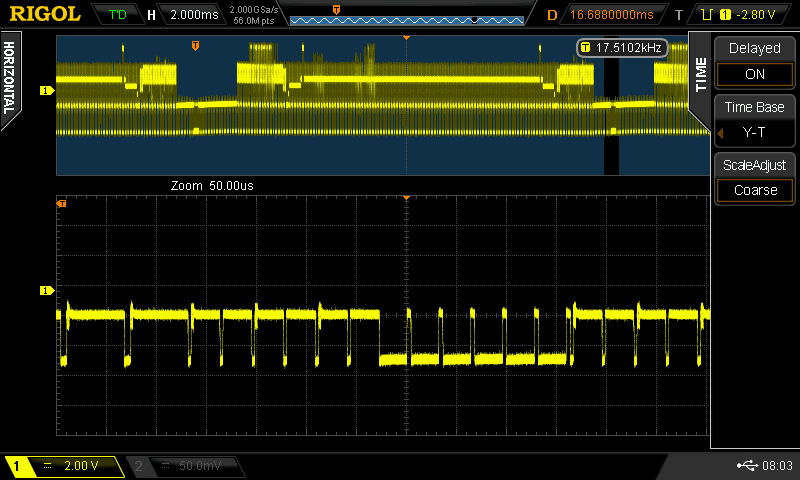
\includegraphics[width=1.0\linewidth]{images/scope/framerate-scope.png}
	\caption[Scope frame rate]{Frame duration as measured with a scope from a \textit{Model 1 VA3 system}.}
	\label{fig:frameratescope}
\end{figure}

The oscilloscope shows a frame duration of \textit{16.888}\ac{ms}, and this is the value used in the configuration file\footnote{Described in appendix \ref{mfnconfig}.} for the initial frame rate calculations.

After the \textit{sync pulses} are detected\footnote{Described in appendix \ref{mfnconfig}.}, a new frame rate value is calculated from the audio file. This new frame rate is used across the whole process, and can vary from the vintage console due to a combination of different reasons.

Every audio card can have a slightly different \textit{sample clock}\footnote{See appendix \ref{audiocards}.}, and this variation will affect the starting and ending points within the recording. Such variation can be detected and estimated from the audio signal, and it is reported if the \textit{verbose log}\footnote{See section \ref{verbose}.} option is enabled.

The selected \textit{sample rate} for recording can also affect the \textit{sample clock} precision even while using the same card\footnote{This is the case when using the \textit{M-Audio 192} \cite{maudio} in \hz{44100}, but when using \hz{48000} the sample clock is spot on.}.

The most important case, and the one for which the \textit{sync pulse} solution was implemented, is when comparing a modern system such as an \textit{emulator} or a \ac{fpga} implementation. These usually run at modern \textit{refresh rate}\footnote{The refresh rate is the inverse of the frame rate. For example with \textit{16.888} it would be $\sfrac{1}{16.888}$ which is \textit{59.92 frames per second}.} for better compatibility with current display technology, such as \textit{HDTVs}, since the vintage hardware has \textit{refresh rates} that are slightly off-spec\footnote{\ac{ntsc} is \textit{59.97 frames per second}.}.

Since \textit{frame rates} differ and the system uses the frame rate as a master clock for program execution, the resulting audio recordings also have a difference in length. For example when using an implementation adjusted for \ac{ntsc}, there is a \textit{0.001} second difference in each block of 20 frames. Although this seems to be negligible, it adds. In a one minute recording, such as the ones used for \textit{MDFourier}, every note was misaligned due to this difference.

The software discards the extra duration in these cases, adjusting for fractions of a second every time they reach the next sample. Since the notes are not played during the whole 20 frames and the window filters help to compensate the signals, the comparison is perfectly aligned for the tests. The reader can verify these results via the \textit{MDWave}\footnote{See appendix \ref{mdwave}.} tool.

\chapter{Stereo Audio Balancing}
\label{stereobalancing}

Sometimes the audio recording has different amplitude levels between the right and left audio channels, this is referred to as \textit{stereo imbalance}. Whenever possible, \textit{MDFourier} detects and auto compensates this imbalance in order to give a more uniform graph result. The default behavior can be disabled if desired with option \textit{-B}\footnote{See appendix \ref{extracommand} for details on how to use \textit{extra commands.}}.

This should only be a concern if an imbalance in the source system is suspected. 

\section{Possible causes}

Two causes for imbalance have been identified. At the time of analysis \textit{MDFourier} cannot possibly discern between them, and both can be present at the same time. 

\begin{itemize}
	\item Amplification deficiencies: The system being recorded has an imbalance due to aging capacitors or other issues in its internal amplification circuitry.
	\item Sound card balance: Another common source is caused by imbalance while capturing the audio data. This is regularly present in USB audio cards that have individual knobs to adjust gain per channel as shown in Figure \ref{fig:lexiconknobs}.
\end{itemize}

It must be noted that the internal \textit{PCI audio card}\footnote{See appendix \ref{audiocards} for information regarding \textit{audio cards}.} used during testing has minimal audio imbalance\footnote{In this case the detected unbalance is \textit{0.0018\%} in average.}, and this allows detecting \textit{system amplification deficiencies} with consistency.

\begin{figure}[H]
	\centering
	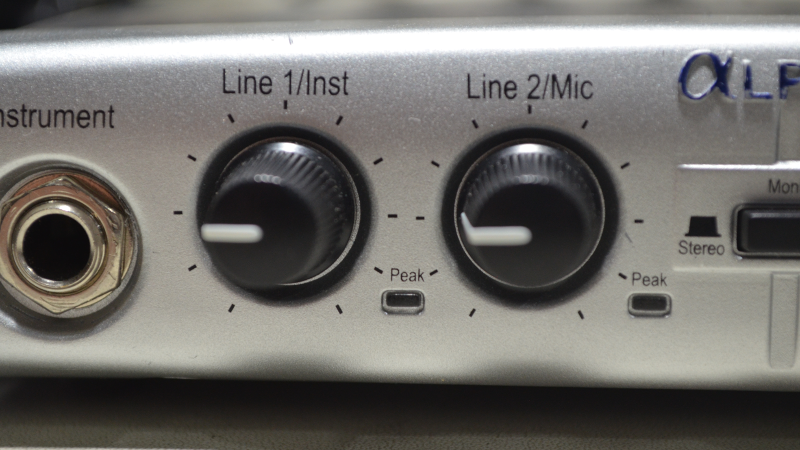
\includegraphics[width=0.8\linewidth]{images/imbalance/lexicon.png}
	\caption[Lexicon knobs]{Lexicon Alpha volume knobs.}
	\label{fig:lexiconknobs}
\end{figure}

The sound card balance issue can be minimized by adjusting the knobs carefully. \textit{MDFourier} can be useful for compensating this via repeated testing, since any imbalance is reported in the output. It has also been found that leaving gain at zero in some cards, like the \textit{M-Track}, produces more pronounced imbalance than at \textit{50\%}. However this requires recording from a source that is known to be balanced.

\begin{figure}[H]
	\centering
	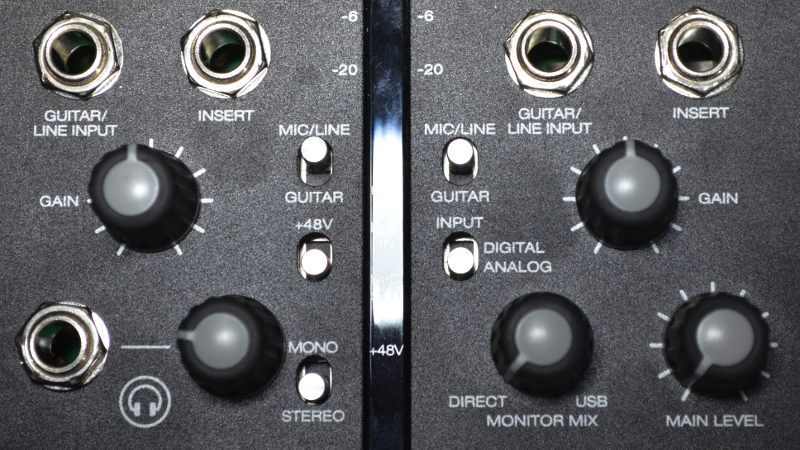
\includegraphics[width=0.8\linewidth]{images/imbalance/mtrack.png}
	\caption[M-Track knobs]{M-Track volume knobs at 50\%.}
	\label{fig:mtrackknobs}
\end{figure}

In order to detect and compensate audio imbalance, at least one \textit{monaural} block must exist within the \textit{mfn}\footnote{See appendix \ref{mfnconfig} for details.} configuration profile being used.

The software assumes that the monaural signal must be the exact same amplitude between left and right audio channels, and compensates by normalizing the \textit{samples} from one unbalanced channel by adjusting them via the proportional ratio. 

\chapter{Differences due to temperature}

During the initial development of the software there was a single instance where unexpected variations were present between different recordings of the same hardware using the same audio capture card as shown in Figure \ref{fig:heatdiff}.

\begin{figure}[H]
	\centering
	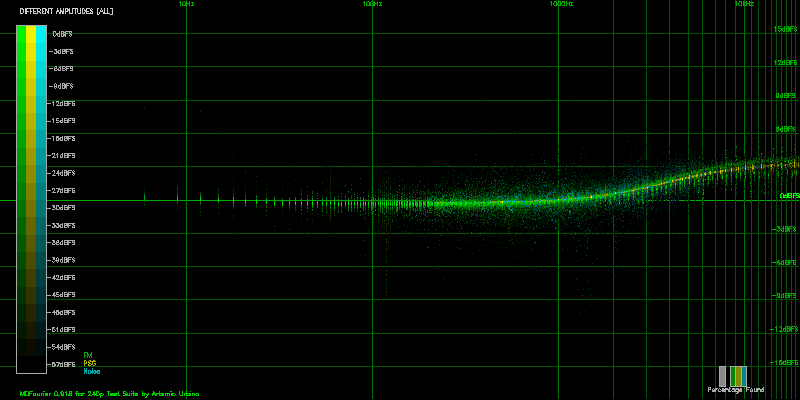
\includegraphics[width=1.0\linewidth]{images/heat/0-plotheat.png}
	\caption[Heat Difference]{Audio difference caused by heat in \textit{Model 1 VA3 system}.}
	\label{fig:heatdiff}
\end{figure}

After analysis, it was found that the difference was present only in the left channel and was caused by a severe difference in temperature while recording. The room was at $29^\circ$C\footnote{$84.2^\circ$F.} as shown in Figure \ref{fig:heatroomtemp}, and the \textit{Sega Genesis Model 1 VA3} under testing had been powered on for around 30 minutes.

\begin{figure}[H]
	\centering
	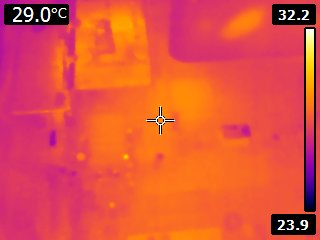
\includegraphics[width=0.4\linewidth]{images/heat/1-roomtemp.jpg}
	\caption[Room temperature]{Console at room temperature \textit{Model 1 VA3 system}.}
	\label{fig:heatroomtemp}
\end{figure}

At first warm up differences were suspected, but after some cooling, \textit{cold boot}\footnote{Powering on the console after it had cool down, and immediately making the recording.} and measurements using a thermal camera it was determine that the room temperature on top of the warm up was the culprit, since the results could not be replicated when the room had cooled down to $22^\circ$C\footnote{$71.6^\circ$F.}. 

In order to replicate the results, its vents were obstructed to prevent heat dissipation\footnote{Ventilation were covered with electrical tape.} for a brief period. The results could be replicated at will under these conditions after just a few minutes of use.

It must be noted that the temperature of the headphone amplifier\footnote{CXA1034} of the console reaches $82.9^\circ$C\footnote{$181.22^\circ$F.} with cover removed as shown in Figure \ref{fig:heathigh}, so higher temperatures are expected with it closed. This is important since some of the stock capacitors around the headphone amplifier are radiated due to proximity, and can probably reach temperatures beyond their intended rating in warm climates.

\begin{figure}[H]
	\centering
	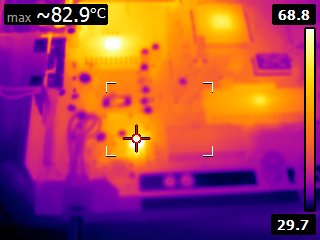
\includegraphics[width=0.4\linewidth]{images/heat/2-hot.jpg}
	\caption[Hot Console]{\textit{Model 1 VA3 system} with amp at $80^\circ$C.}
	\label{fig:heathigh}
\end{figure}

\chapter{Corner cases}
\label{cornercase}

While testing the default\textit{ frequency domain} normalization\footnote{See appendix \ref{normalization}.}, I found that one artificially generated case would produce results that were unexpected and surprising. After analysis, I believe them to be the correct handling of the data, and the appropriate comparison results.

For this example we'll modify a file as detailed in \textit{Scenario 3}\footnote{See section \ref{scenario3}.}, but this time a \khz{1z} \db{6} tone will be added instead of the \hz{500} from that previous case.

I was expecting the result detailed in \textit{Scenario 3}, but was greeted with the graph shown in Figure \ref{fig:corner1}:

\begin{figure}[H]
	\centering
	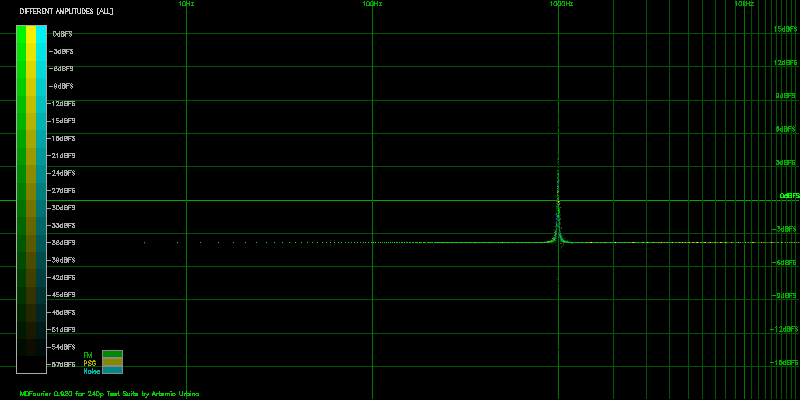
\includegraphics[width=1.0\linewidth]{images/corner/plot1.png}
	\caption[Corner Case 1]{Signal compared to itself with \khz{1} \db{6} artificially inserted.}
	\label{fig:corner1}
\end{figure}

I thought it was a bug in the processing of \textit{frequency domain normalization}. But after careful analysis, this is the correct result from such process.

It is all due to a big coincidence: the maximum global \textit{amplitude} of the original signal used for this scenario is located at \hz{1005.99}, at just \hz{5.99} from the \khz{1} peak that was artificially inserted. As you might sharply point out, figure \ref{fig:corner1} doesn't show the peak \db{6} below zero. But that is because it is not centered at \hz{1005.99}. 

Here is the result when centering the peak at \hz{1005.99}:

\begin{figure}[H]
\centering
\includegraphics[width=1.0\linewidth]{images/corner/plot2.png}
\caption[Corner Case 2]{Signal compared to itself with \khz{1005.99} \db{6} artificially inserted.}
\label{fig:corner2}
\end{figure}

Now the majority of the curve is \db{6} below zero, and the peak is at zero. But  why?

As explained in appendix \ref{normalization}, the process of frequency normalization consists in finding the highest amplitude in the signal and use that as a reference point for matching both signals. In this case, both signals have their maximum at \hz{1005.99}, but we also modified the \textit{comparison} file to have a \db{6} \hz{1005.99} peak. As a result when using the original \textit{reference} file as a model and judging the \textit{comparison} file against it, the rest of the signal has been lowered from this perspective.

This would mean that if two systems had these audio signatures, the resulting graph would tell us that the \textit{comparison} console is--in general--producing the frequencies at lower amplitudes. If the \textit{comparison} system had to be modified to match the reference system, the rest of the frequencies in the signal should be raised by \db{6}, since the single point at \hz{1005.99} already matches the reference signal. It is just a matter of perspective. It helps keeping in mind that \textit{MDFourier} does relative comparisons, and in this framework the \textit{reference} file is the absolute model.

In case we'd like to see a graph that would probably be easier to digest--but which I now believe is not as accurate in representing the relative differences--one could enable the \textit{time domain normalization}. The resulting graph would be the familiar now result from figure \ref{fig:corner3}:

\begin{figure}[H]
	\centering
	\includegraphics[width=1.0\linewidth]{images/corner/plot3.png}
	\caption[Corner Case 3]{Signal compared to itself with \hz{1005.99} \db{6} artificially inserted, but normalized in the time domain.}
	\label{fig:corner3}
\end{figure}

This graph tells us the exact same thing: if the \textit{comparison} signal is to be modified to match the \textit{reference} signal, the peak at \hz{1005.99} must be lowered by \db{6}. Since the results in both cases would be the same, both interpretations are equivalent.
	
However, I am inclined to adopt the first position, since it has an absolute reference point. Whereas the second graph and interpretation must be modified depending on the input. For this second scenario to work, our framework needs to be modified for special cases--that are highly unlikely to be found in the wild. And since that creates unnecessary inconsistencies and results in imprecision, the \textit{time domain normalization} is not used by default.

\chapter{Known Issues}

I'm positive several deficiencies in my implementation still elude me. However here are a few I'm aware of and have not addressed yet.

\begin{itemize}
	\item \ac{pcm} generated by the \textit{FM} chip is not covered in the current \textit{Mega Drive/Sega Genesis} implementation. It is assumed the response will follow the \textit{YM2612} curve.
	\item A better signal could  be generated to cover either more or specific cases.
	\item When comparing \textit{Mega CD/Sega CD}, the \textit{\ac{cdda}} block uses the detected \textit{frame rate} for the comparison. It should use the expected one from the configuration file instead, even when comparing to an \textit{emulator/FPGA}. This causes slight ringing in the results, but they are at least \textit{95\%} correct.
	\item The \ac{pcm} chip from the \textit{Mega CD/Sega CD} is not yet implemented in the tests, since it's behavior is expected t follow the same amplification path that \textit{CD-DA} does. It might have differences in balance, though.
\end{itemize}

Please contact me if you are aware of any details that I have missed.\footnote{See appendix \ref{contact}.}

\chapter{Window Function equations and graphs}
\label{windowfunctiondetails}

This appendix lists the equation and curve of each \textit{Window Function} used to limit \textit{spectral leakage} as described in section \ref{windows}.

\section{Tukey}

The default is a \textit{Tukey} window selected for this purpose. It uses $\alpha = 0.6$, zeroing just a few samples, with minimal \textit{spectral leakage} and good amplitude response.

The following equation is used to create the slopes:

\begin{equation}
tukey(x)=\frac{1}{2}(1+\cos(\frac{\pi(|x-\frac{N-1}{2}|-\alpha \frac{N-1}{2})}{(1-\alpha)\frac{N-1}{2}}))
\end{equation}

And this is the resulting graph of the \textit{Tukey} window, ranges are \textit{0.0} to \textit{1.0} horizontally and \textit{-0.1} to \textit{1.1} vertically.

\begin{figure}[H]
	\centering
	\includegraphics[width=0.4\linewidth]{images/windows/window-tukey.png}
	\caption[Tukey Window]{Tukey window used by \textit{MDFourier}, vertical lines are frames on a 20 frame signal.}
	\label{fig:window-tukey}
\end{figure}

Detailed information can be found in the reference webpage \cite{tukey}.

\section{Hann}
When selected, a typical \textit{Hann} window is used. This should be used to get the last \textit{spectral leakage}, with a very small trade off in amplitude accuracy.

\begin{equation}
hann[x] = \frac{1}{2}(1 - \cos(\frac{2\pi(x+1)}{n+1}))
\end{equation}

\begin{figure}[H]
	\centering
	\includegraphics[width=0.4\linewidth]{images/windows/window-hann.png}
	\caption[Hann Window]{Hann Window.}
	\label{fig:window-hann}
\end{figure}

\section{Flattop}
A typical \textit{Flat top} window is used, selecting this will target amplitude accuracy against frequency bin precision.

\begin{align*}
flattop(x)=0.21557895 - 0.41663158\cos(2\pi\frac{x}{n-1})+ 0.277263158\cos(4\pi\frac{x}{n-1})\\
- 0.083578947\cos(6\pi\frac{x}{n-1}) + 0.006947368\cos(8\pi\frac{x}{n-1})
\end{align*}

\begin{figure}[H]
	\centering
	\includegraphics[width=0.4\linewidth]{images/windows/window-flattop.png}
	\caption[Flat Top window]{Flat Top window.}
	\label{fig:window-flattop}
\end{figure}

\section{Hamming}
A typical \textit{Hamming} window is used, presented for completeness and reference since the samples are never zeroed out.

\begin{equation}
hamming[x] = 0.54 - 0.46\cos(\frac{2\pi x}{n-1})
\end{equation}

\begin{figure}[H]
	\centering
	\includegraphics[width=0.4\linewidth]{images/windows/window-hamming.png}
	\caption[Hamming window]{Hamming window.}
	\label{fig:window-hamming}
\end{figure}

\section{No Window}

No window is applied to the signal before applying the \ac{dft}, equivalent to a \textit{rectangular window}. This leaves the signal unprocessed and any uncontrolled decay and audio card noise will be factored in as part of the periodic signal.

There is more information on windows and their usage in the reference webpage \cite{windowtypes}.

\chapter{Color Filter Function details}
\label{filterfunctions}

This appendix contains a description, graph and example of each \textit{Color Filter Function} from section \ref{colorfilter}.

\section{None} 

No filtering is applied, as a result all differences are plotted with the brightest color. 

\begin{figure}[H]
	\centering
	\includegraphics[width=0.4\linewidth]{images/colorfilter/BetaFunctionPlot_0.png}
	\caption[No Filter]{No Filter.}
	\label{fig:betafunctionplot0}
\end{figure}

\begin{figure}[H]
	\centering
	\includegraphics[width=1\linewidth]{images/colorfilter/BetaFunctionPlot_0_Data.png}
	\caption[No Filter]{No Filter Applied.}
	\label{fig:betafunctionplot0data}
\end{figure}

\section{$\sqrt{\textit{\acrshort{dbfs}}}$} 

A square root function will only attenuate the lowest amplitude differences.

\begin{figure}[H]
	\centering
	\includegraphics[width=0.4\linewidth]{images/colorfilter/BetaFunctionPlot_1.png}
	\caption[Square Root filter]{Square Root filter.}
	\label{fig:betafunctionplot1}
\end{figure}

\begin{figure}[H]
	\centering
	\includegraphics[width=1\linewidth]{images/colorfilter/BetaFunctionPlot_1_Data.png}
	\caption[Square Root filter]{Square Root filter Applied.}
	\label{fig:betafunctionplot1data}
\end{figure}

\section{$\beta(3,3)$}

A Beta Function filter with parameters (3, 3) will attenuate a bit more from the lower range, still showing most of the differences.

\begin{figure}[H]
	\centering
	\includegraphics[width=0.4\linewidth]{images/colorfilter/BetaFunctionPlot_2.png}
	\caption[Beta Function(3,3)]{Beta Function(3,3).}
	\label{fig:betafunctionplot2}
\end{figure}

\begin{figure}[H]
	\centering
	\includegraphics[width=1\linewidth]{images/colorfilter/BetaFunctionPlot_2_Data.png}
	\caption[Beta Function(3,3)]{Beta Function(3,3) Applied.}
	\label{fig:betafunctionplot2data}
\end{figure}

\section{Linear} 

The linear function is the default, and has no bias. Half the dinamic range corresponds to half the color rage.

\begin{figure}[H]
	\centering
	\includegraphics[width=0.4\linewidth]{images/colorfilter/BetaFunctionPlot_3.png}
	\caption[Linear]{Linear Function.}
	\label{fig:betafunctionplot3}
\end{figure}

\begin{figure}[H]
	\centering
	\includegraphics[width=1\linewidth]{images/colorfilter/BetaFunctionPlot_3_Data.png}
	\caption[Linear Applied]{Linear Function Applied.}
	\label{fig:betafunctionplot3data}
\end{figure}

\section{$\textit{\acrshort{dbfs}}^2$}

A squared function will attenuate a lot more differences, as a result frequencies with the highest amplitude in the reference signal will be brighter.

\begin{figure}[H]
	\centering
	\includegraphics[width=0.4\linewidth]{images/colorfilter/BetaFunctionPlot_4.png}
	\caption[Linear]{Linear Function.}
	\label{fig:betafunctionplot4}
\end{figure}

\begin{figure}[H]
	\centering
	\includegraphics[width=1\linewidth]{images/colorfilter/BetaFunctionPlot_4_Data.png}
	\caption[Linear Applied]{Linear Function Applied.}
	\label{fig:betafunctionplot4data}
\end{figure}

\section{$\beta(16,2)$} 

A Beta Function filter with parameters (16,2) will attenuate almost all the differences, and only the frequencies with the highest amplitude in the reference signal will be brighter.

\begin{figure}[H]
	\centering
	\includegraphics[width=0.4\linewidth]{images/colorfilter/BetaFunctionPlot_5.png}
	\caption[Beta Function(16,2)]{Beta Function(16,2).}
	\label{fig:betafunctionplot5}
\end{figure}

\begin{figure}[H]
	\centering
	\includegraphics[width=1\linewidth]{images/colorfilter/BetaFunctionPlot_5_Data.png}
	\caption[Beta Function(16,2)]{Beta Function(16,2) Applied.}
	\label{fig:betafunctionplot5data}
\end{figure}

\chapter{Requirements}
\label{requirements}
\section{Audio capture device}
\label{audiocards}
For capturing the audio files, an \textit{audio capture device} is needed. It is recommended to use a musical grade \textit{audio card} in order to get a \textit{flat frequency} response across the human hearing spectrum. Fortunately, these devices have become more affordable.

So far four audio cards have been used in my personal setup. The sample recordings available for download\footnote{See appendix \ref{downloads}.} were made with three cards of them, a complete set with each one of them.

I have no association or business relationship with these products, they are just presented as  working examples. As more people use the software and we--as a community--compare files, this list can be expanded with recommendations.

\begin{itemize}
	\item \textbf{Lexicon Alpha:} An USB audio card\footnote{Uses a CS4270 24-Bit, 192 kHz Stereo Audio CODEC and a TAS1020B for USB communications. Verified by opening the device. \cite{lexicon}.}. 
	\item \textbf{M-Audio M-Track:} A USB audio card\footnote{Uses a CS5341  105 dB, 192 kHz, Multi-Bit Audio A/D Converter and a TAS1020B for USB communications. Verified by opening the device. \cite{maudiomtrack}.}. 
	\item \textbf{M-Audio M-Track Pro:} A USB audio card, adds \define{spdif} over the regular model\footnote{Not opened for component verification, but assumed to use the same components as the regular version.}. \cite{maudiomtrack}
	\item \textbf{M-Audio Audiophile 192:} An internal audio card\footnote{Uses a VT1720 Envy24PT PCI Multi-Channel Audio Controller.} that is no longer available in the market \cite{maudio}
\end{itemize}

Some cards marketed for podcasting and audio cassette digitization were tested\footnote{Gear of this type could exist with a \textit{flat frequency} response, current technology should allow any product to offer this basic requirement. But alas, the ones we've tested failed in our tests.}, but they didn't show a flat frequency response. You should try to use a sound card that is aimed to musicians or instrument recording.

\subsection{Sampling clocks}
\label{samplingclocks}

Sound cards have their own internal clock for sampling\footnote{For more details, see \cite{SoundCardClock} \cite{soundcardtiming} \cite{gwsoundcardtiming}.}, which can sometimes deviate enough so that \textit{MDFourier} can report \textit{frame rate} differences. From my tests, this is more prominent when using the \khz{44.1} sample rate, and minimized when using \khz{48}. The effect is compensated for while loading the file and during trimming, so it shouldn't be a problem  due to the small variations this produces in the frequency domain. 

\section{Computer}

Any computer and operation system can be used if you are compiling the \textit{source code} from scratch\footnote{See appendix \ref{downloads} for download links.}, but a statically linked \textit{Microsoft Windows executable} is provided for convenience, alongside a \textit{front end}. See chapter \ref{usinggui} for instructions on using the \ac{gui}.

\section{Game Consoles or emulators}

You'll need either the provided example audio files\footnote{See appendix \ref{downloads} for download urls.} or to create your own, by recording from your own source. This is probably the desired route, since you will want to compare against your files.

\section{Flash cart, or means to run the \textit{Tone Generator}}

The console needs to run the \textit{Tone Generator} created for that platform--which are provided with the rest of \textit{MDFourier}. If possible this will be integrated into each version of the \textit{240 test suite} \cite{240pSuite}.

In order to run these, you'll either need a \textit{flash cart} or a custom loading solution compatible with the target platform.

\section{Cables and adapters}

You'll need cables--and maybe some adapters--to connect the audio output from the console to the input of your \textit{audio capture card}.

\section{Audio capture software}

Your \textit{audio capture card} will probably be bundled with some audio editing software, or you can use \textit{Audacity} \cite{audacity} or \textit{Goldwave} \cite{goldwave} depending on your operating system.

\chapter{Compiling from source code}

\section{Dependencies}

\textit{MDFourier} needs a few libraries to be compiled. In \textit{Linux}, \textit{UN*X} based systems and \textit{Cygwin} \cite{cygwin}; you can link it against the latest versions of the libraries. 

\begin{itemize}
	\item Fastest Fourier Transform in the West. (fftw) \cite{fftw}
	\item The GNU plotutils package. \cite{libplot}
	\item \ac{png} Reference Library: libpng. \cite{libpng}
	\item \ac{flac} Reference Library: libFLAC. \cite{libflac}
\end{itemize}

The following implementations are also used and included with the source files:

\begin{itemize}
	\item sort.h for tim sort. \cite{sort}
	\item Incomplete Beta Function. \cite{betafunction}
\end{itemize}

The pre-compiled executable of the \textit{Analysis Software} for \textit{Windows} is created with \textit{MinGW}\cite{mingw}, and statically linked for distribution against these libraries:

\begin{itemize}
	\item fftw-3.3.8 \cite{fftw}
	\item plotutils-2.6 \cite{libplot}
	\item libpng-1.5.30 \footnote{This older version was used to simplify the build process in this statically linked executable. Sources at \url{https://sourceforge.net/projects/libpng/files/libpng15/1.5.30/}.}
\end{itemize}

The \textit{makefiles} to compile either version are provided with the source code \cite{sourcecode}.

\chapter{Colors available for graphs}
\label{availablecolors}

This is the list of colors that can be used in the \textit{MFN configuration file} described in appendix \ref{mfnconfig}: 

\begin{itemize}
	\item red
	\item green
	\item blue
	\item yellow
	\item magenta
	\item aqua
	\item orange
	\item purple
\end{itemize}

\chapter{Licensing}
\label{license}

\textit{MDFourier} Copyright (C)2019 Artemio Urbina

This program is free software: you can redistribute it and/or modify
it under the terms of the GNU General Public License as published by
the Free Software Foundation, either version 3 of the License, or
(at your option) any later version.

This program is distributed in the hope that it will be useful,
but WITHOUT ANY WARRANTY; without even the implied warranty of
MERCHANTABILITY or FITNESS FOR A PARTICULAR PURPOSE.  See the
GNU General Public License for more details.

You should have received a copy of the GNU General Public License
along with this program.  If not, see \url{https://www.gnu.org/licenses/}.	

\chapter{Contact the author}
\label{contact}

You can contact me via twitter \url{http://twitter.com/Artemio} or e-mail me at \textit{aurbina@junkerhq.net}.

\chapter{Acknowledgments}

I'd like to thank the following people for helping me so these tools could be completed. First and foremost to my family, who helped me find the time to learn and make progress.

\end{appendices}

\begin{thebibliography}{9}
	\bibitem{FourierTransformApps}
	Bracewell, Ronald N. 
	\textit{The Fourier Transform and Its Applications (2 ed.).}
	McGraw-Hill. ISBN 978-0-07303938-1.
	
	\bibitem{genesisaudio}
	Ace, \textit{GUIDE: A complete overview of the many Sega Genesis/MegaDrive models}, Sega-16,
	\url{http://www.sega-16.com/forum/showthread.php?7796-GUIDE-Telling-apart-good-Genesis-1s-and-Genesis-2s-from-bad-ones}
	
	\bibitem{genesisaudio2}
	The Best Version of the Genesis, RetroRGB
	\url{https://www.retrorgb.com/genesisversions.html}
	
	\bibitem{genesishw}
	Sega Mega Drive/Hardware revisions, Sega Retro,
	\url{https://segaretro.org/Sega_Mega_Drive/Hardware_revisions}
	
	\bibitem{sourcecode}
	Github,
	\textit{MDFourier source code C99},
	\url{https://github.com/ArtemioUrbina/MDFourier/}.
	
	\bibitem{240pSuite}
	240p test Suite,
	\textit{Wiki web page},
	\url{http://junkerhq.net/240p/}.
	
	\bibitem{fftw}
	Fastest Fourier Transform in the West.,
	\textit{web page},
	\url{http://fftw.org/}.
	
	\bibitem{libpng}
	libPNG,
	\textit{web page},
	\url{https://libpng.sourceforge.io/}
	
	\bibitem{libflac}
	libFLAC,
	\textit{web page},
	\url{https://xiph.org/flac/}
	
	\bibitem{libplot}
	GNU Plot Utils,
	\textit{web page},
	\url{https://www.gnu.org/software/plotutils/}
	
	\bibitem{sort}
	An implementation of a ton of sorting algorithms in C with a user-defined type,
	\textit{web page},
	\url{https://github.com/swenson/sort/}
	
	\bibitem{dbdiff}
	\textit{Human Hearing: Amplitude Sensitivity}, 
	Mark Sanfilipo — April 04, 2005,
	\url{https://www.audioholics.com/room-acoustics/human-hearing-amplitude-sensitivity-part-1}
	
	\bibitem{betafunction}
	incbeta, 
	\textit{Incomplete Beta Function in C},
	\url{https://codeplea.com/incomplete-beta-function-c/}.
	
	\bibitem{windowtypes}
	Window Types: Hanning, Flattop, Uniform, Tukey, and Exponential ,
	\textit{web page},
	\url{https://community.plm.automation.siemens.com/t5/Testing-Knowledge-Base/Window-Types-Hanning-Flattop-Uniform-Tukey-and-Exponential/ta-p/445063/}.
	
	\bibitem{dbfs}
	dB Full Scale, 
	\url{https://www.sweetwater.com/insync/dbfs/}
	
	\bibitem{SoundCardClock}
	Sound Card Sampling clock variation
	\url{http://www.stu2.net/wiki/index.php/Calibrate_Sound_Card/}
	
	\bibitem{soundcardtiming}
	So how accurate is a typical PC sound card? How stable is the output? How would one measure this?
	Experiments with a PC sound card by leapsecond
	\url{http://www.leapsecond.com/pages/sound-1pps/}
	
	\bibitem{gwsoundcardtiming}
	Each sound card has it's own sampling clock, Goldwave support forums
	\url{http://www.goldwave.ca/forums/viewtopic.php?p=17470}
	
	\bibitem{MontyMontgomery}
	D/A and A/D | Digital Show and Tell (Monty Montgomery @ xiph.org)
	\url{https://www.youtube.com/watch?v=cIQ9IXSUzuM}
	
	\bibitem{leakage}
	Harris, Fredric j. (Jan 1978). \textit{"On the use of Windows for Harmonic Analysis with the Discrete Fourier Transform"}. Proceedings of the IEEE. 66 (1): 51–83.
	\url{https://web.mit.edu/xiphmont/Public/windows.pdf}
	
	\bibitem{zeropaddinginterpolate}
	Spectral Leakage and Zero-Padding of the Discrete Fourier Transform
	\url{https://dspillustrations.com/pages/posts/misc/spectral-leakage-zero-padding-and-frequency-resolution.html}
	
	\bibitem{ZeroPaddingBad}
	Why is it a bad idea to filter by zeroing out FFT bins?
	\url{https://dsp.stackexchange.com/questions/6220/why-is-it-a-bad-idea-to-filter-by-zeroing-out-fft-bins}
	
	\bibitem{mingw}
	MinGW, 
	\textit{Minimalist GNU for Windows},
	\url{http://mingw.org/}.
	
	\bibitem{cygwin}
	Cygwin,
	\textit{a large collection of GNU and Open Source tools which provide functionality similar to a Linux distribution on Windows.}
	\url{https://www.cygwin.com/}
	
	\bibitem{tukey}
	Tukey window, Recording Blogs
	\url{https://www.recordingblogs.com/wiki/tukey-window}
	
	\bibitem{maudio}
	M-Audio Audiophile 192,
	\textit{Specifications},
	\url{https://www.soundonsound.com/reviews/m-audio-audiophile-192/}.
	
	\bibitem{lexicon}
	Lexicon Alpha USB card,
	\textit{Product web page},
	\url{https://lexiconpro.com/en/products/alpha/}.
	
	\bibitem{maudiomtrack}
	M-Audio M-Track USB card,
	\textit{Product web page},
	\url{	https://www.m-audio.com/products/view/m-track}.
	
	\bibitem{audacity}
	Audacity
	\textit{web page},
	\url{https://www.audacityteam.org/}.
	
	\bibitem{goldwave}
	Goldwave
	\textit{product web page},
	\url{https://www.goldwave.com/}.
	
	\bibitem{sma}
	Adam Hayes, Simple Moving Average - SMA Definition
	\url{https://www.investopedia.com/terms/s/sma.asp}
	
	\bibitem{humanvoice}
	Human Speech Spectrum, Frequency Range, Formants, 
	\textit{web site},
	\url{http://www.bnoack.com/index.html?http&&&www.bnoack.com/audio/speech-level.html}.
	\bibitem{noiselevels}
	Noise Level Chart, \textit{web site},
	\url{https://www.noisehelp.com/noise-level-chart.html}
	
	\bibitem{bass}
	Audio Spectrum Explained
	\textit{web site},
	\url{https://www.teachmeaudio.com/mixing/techniques/audio-spectrum/}.
\end{thebibliography}

\printglossaries

\end{document}
